\documentclass[review,authoryear]{elsarticle}

% === PACKAGES ===
\usepackage[utf8]{inputenc}
\usepackage[T1]{fontenc}
\usepackage{geometry}
\geometry{a4paper, margin=2.5cm}
\usepackage{amsmath,amssymb}
\usepackage{graphicx}
\usepackage{booktabs}
\usepackage{multirow}
\usepackage{longtable}
\usepackage{tabularx}
\usepackage{hyperref}
\usepackage{xcolor}
\usepackage{tikz}
\usepackage{pgfplots}
\pgfplotsset{compat=1.17}
\usepackage{tcolorbox}
\usepackage{algorithm}
\usepackage{algorithmic}
\usepackage{enumitem}
\usepackage{lineno}
\usepackage{caption}
\usepackage{float}
\usepackage{siunitx}
\usepackage{array}
\usepackage{soul}

\usetikzlibrary{shapes,arrows,positioning,calc,fit,backgrounds,decorations.pathreplacing}

\linenumbers

\biboptions{authoryear}

\journal{Earth-Science Reviews}

\begin{document}

\begin{frontmatter}

\title{Graph Neural Networks for Earthquake Early Warning: A Comprehensive Review of Methods, Applications, and Future Directions}

\author[inst1,inst2]{Ahmad R. Purnama\corref{cor1}}
\ead{ahmad.purnama@ft.undip.ac.id}
\author[inst1]{Wei Zhang}
\author[inst2]{Hiroshi Tanaka}
\author[inst3]{Maria C. Rodriguez}

\cortext[cor1]{Corresponding author}

\affiliation[inst1]{organization={Department of Computer Science, Faculty of Engineering, Universitas Diponegoro},
  city={Semarang},
  country={Indonesia}}
\affiliation[inst2]{organization={Department of Earth Sciences, Faculty of Natural Sciences, Universitas Diponegoro},
  city={Semarang},
  country={Indonesia}}
\affiliation[inst3]{organization={Institute of Geophysics, National Seismological Center},
  city={Santiago},
  country={Chile}}

\begin{abstract}
Earthquake Early Warning (EEW) systems provide seconds to tens of seconds of advance notice before destructive ground shaking arrives at a target site. Traditional approaches rely on empirical scaling relationships and threshold-based detection algorithms that exhibit well-documented limitations in accuracy, speed, and robustness, particularly for large-magnitude events and sparse network geometries. Graph Neural Networks (GNNs) offer a paradigm shift by natively representing seismic monitoring networks as graphs, where stations constitute nodes and spatial relationships define edges. This graph-structured representation enables explicit modeling of inter-station correlations, wavefield propagation patterns, and network topology effects that are fundamental to seismological analysis but difficult to capture with conventional architectures.

This review systematically examines GNN methodologies for EEW, covering architectures from spectral methods (GCN) to spatial approaches (GAT, GraphSAGE) and temporal-spatial formulations. We analyze applications spanning seismic phase picking, event detection, source characterization, magnitude estimation, ground motion prediction, and source localization. Detailed comparisons against traditional methods (STA/LTA, template matching) and deep learning baselines (PhaseNet, EQTransformer) demonstrate that GNN approaches achieve measurable improvements, particularly for sparse networks and complex multi-event sequences. We examine benchmark datasets (STEAD, INSTANCE, LEN-DB), identify critical challenges including real-time processing constraints, transfer learning across tectonic regions, and model interpretability, and outline future directions encompassing physics-informed GNNs, foundation models for seismology, federated learning, and edge computing deployment. This review provides researchers and practitioners with a comprehensive roadmap for advancing GNN-based EEW systems toward operational deployment.
\end{abstract}

\begin{keyword}
Graph Neural Networks \sep Earthquake Early Warning Systems \sep Seismology \sep Deep Learning \sep Seismic Network \sep Ground Motion Prediction \sep Phase Picking \sep Spatio-temporal Modeling
\end{keyword}

\end{frontmatter}

\newpage

%% ============================================================
%% SECTION 1: INTRODUCTION
%% ============================================================
\section{Introduction}
\label{sec:introduction}

Earthquakes remain among the most devastating natural hazards, causing significant loss of life, infrastructure damage, and economic disruption worldwide. The 2011 Tohoku earthquake (M$_w$ 9.0) in Japan resulted in over 15,000 fatalities and triggered a catastrophic tsunami \citep{simons2011decade}, while the 2023 Turkey-Syria earthquake sequence (M$_w$ 7.8) caused more than 50,000 deaths across a wide region. These events underscore the persistent vulnerability of human populations to seismic hazards and highlight the critical importance of effective early warning systems that can provide precious seconds of advance notice before destructive shaking arrives.

Earthquake Early Warning (EEW) systems exploit the differential propagation velocities of seismic waves---specifically, the faster but less destructive P-waves (compressional, $\sim$6 km/s) versus the slower but more damaging S-waves (shear, $\sim$3.5 km/s) and surface waves---to issue alerts before the arrival of strong ground motion at a target site \citep{allen2003potential, allen2012earthquake}. The concept, first proposed in the late 1860s and operationalized in Japan following the development of the UrEDAS system \citep{nakamura1988urgency}, has matured into deployed systems across multiple countries including Japan (JMA), Mexico (SASMEX), the United States (ShakeAlert), Taiwan (CWA), Italy, and others \citep{gasparini2007earthquake, given2018shakealert, hsiao2009development}.

Despite decades of development, existing EEW systems face fundamental limitations. Traditional approaches based on empirical scaling relationships and threshold algorithms (e.g., $\tau_c$-P$_d$ methods) struggle with: (1) the inherent trade-off between speed and accuracy in source characterization; (2) magnitude saturation for large events when using only initial P-wave seconds; (3) high false alert rates in noisy environments; and (4) poor performance in regions with sparse station coverage \citep{satriano2011earthquake, bose2018finder}. These limitations have motivated the seismological community to explore data-driven approaches that can potentially overcome the constraints of physics-based empirical models.

\subsection{The Rise of Deep Learning in Seismology}

The application of deep learning to seismological problems has accelerated dramatically since 2018, building on foundational advances in representation learning \citep{lecun2015deep, krizhevsky2012imagenet, he2016deep} and sequence modeling \citep{hochreiter1997long, graves2013speech, schuster1997bidirectional}. Modern deep learning training relies on key techniques including adaptive optimizers \citep{kingma2015adam}, regularization methods \citep{srivastava2014dropout, ioffe2015batch}, and generative models \citep{goodfellow2014generative, kingma2014auto}. These advances enabled transformative progress in seismic phase picking \citep{ross2018generalized, zhu2019phasenet, mousavi2020earthquake}, event detection \citep{perol2018convolutional, yoon2015earthquake}, earthquake location \citep{kriegerowski2019deep, lomax2012automatic}, and ground motion prediction \citep{derras2014towards}. Architectures such as PhaseNet \citep{zhu2019phasenet} and EQTransformer \citep{mousavi2020earthquake} have demonstrated performance comparable to or exceeding manual analyst picks across diverse tectonic settings, as quantified by standardized benchmarking frameworks such as SeisBench \citep{woollam2022seisbench} and comparative picker evaluations \citep{munchmeyer2022picker}. Comprehensive reviews by \citet{bergen2019machine}, \citet{kong2019machine}, \citet{mousavi2022deep}, and \citet{sahara2023review} document the breadth of machine learning applications in solid Earth geoscience, establishing deep learning as an indispensable tool in modern seismology.

However, most existing deep learning approaches treat seismic stations independently---processing waveforms from individual stations or station triplets through CNNs or RNNs without explicitly modeling the spatial relationships between stations in a network. This station-independent processing paradigm ignores a fundamental aspect of seismological observation: seismic monitoring networks are inherently graph-structured systems where the spatial configuration of stations, their inter-station distances, and the wavefield propagation patterns across the network carry essential information about earthquake sources.

\subsection{Why Graph Neural Networks for Seismology?}

Graph Neural Networks (GNNs) provide a natural computational framework for processing data defined on irregular graph structures \citep{scarselli2009graph, bronstein2017geometric, wu2021comprehensive, zhang2020deep}. Recent theoretical perspectives on message passing architectures \citep{velivckovic2022message} further clarify their representational capabilities. In the context of seismic monitoring, a GNN represents stations as nodes equipped with recorded waveform features, while edges encode spatial relationships (distance, azimuth, geological similarity) between station pairs. The message-passing mechanism intrinsic to GNNs enables each station to aggregate information from neighboring stations, effectively learning how seismic wavefield characteristics evolve across the network topology.

This graph-based representation offers several compelling advantages for EEW applications:

\begin{enumerate}[label=(\roman*)]
  \item \textbf{Network-aware processing}: GNNs naturally incorporate the full network geometry, enabling joint processing of multi-station observations with explicit spatial reasoning about wavefield propagation.
  \item \textbf{Permutation invariance}: GNN architectures are invariant to station ordering, making them robust to network configuration changes (station additions, removals, or failures).
  \item \textbf{Scalability}: GNNs can handle networks of varying sizes without architectural modifications, accommodating both dense urban arrays and sparse regional networks.
  \item \textbf{Dynamic adaptability}: Temporal graph formulations can capture the time-evolving nature of seismic wavefield propagation across station networks.
  \item \textbf{Interpretability}: Attention-based GNN variants can identify which station connections are most informative for specific predictions, providing physically meaningful explanations.
\end{enumerate}

Recent pioneering work has demonstrated the potential of GNNs for seismological applications, including earthquake source characterization \citep{vandenende2020automated}, spatiotemporal event analysis \citep{zhang2021spatiotemporal}, earthquake location and magnitude estimation \citep{mcbrearty2023earthquake}, and phase association \citep{munchmeyer2021gnn}. These studies consistently report improvements over station-independent methods, validating the hypothesis that network-level information processing enhances seismic analysis.

\subsection{Scope and Contributions of This Review}

This review provides the first comprehensive survey dedicated to the intersection of Graph Neural Networks and Earthquake Early Warning systems. While previous reviews have covered machine learning in seismology broadly \citep{mousavi2023review, bergen2019machine, kong2019machine} or GNN methods generally \citep{wu2021comprehensive, zhou2020graph}, none has specifically examined how graph-based deep learning architectures can address the unique challenges of EEW. Our contributions are:

\begin{enumerate}
  \item A systematic taxonomy of GNN architectures and their applicability to different EEW sub-tasks, from phase detection through alert generation.
  \item A critical comparative analysis of GNN-based approaches versus traditional and CNN-based methods across standardized benchmarks.
  \item Identification of key research gaps and technical challenges specific to deploying GNNs in operational EEW contexts.
  \item A forward-looking discussion of emerging paradigms---foundation models, physics-informed GNNs, federated learning---that may shape the next generation of EEW systems.
\end{enumerate}

\subsection{Paper Organization}

The remainder of this review is organized as follows. Section~\ref{sec:eew_fundamentals} presents the fundamentals of earthquake early warning systems, including operational principles, deployed systems worldwide, and technical challenges. Section~\ref{sec:seismic_graphs} discusses the representation of seismic networks as graph-structured data. Section~\ref{sec:gnn_fundamentals} provides a comprehensive overview of graph neural network architectures relevant to seismology. Section~\ref{sec:applications} reviews GNN applications across the EEW processing pipeline. Section~\ref{sec:temporal_spatial} examines temporal-spatial graph network formulations. Section~\ref{sec:comparison} presents comparative analyses with traditional approaches. Section~\ref{sec:benchmarks} surveys benchmark datasets and evaluation protocols. Section~\ref{sec:challenges} discusses challenges and limitations. Section~\ref{sec:future} outlines future research directions. Section~\ref{sec:ethical} addresses ethical and operational considerations. Section~\ref{sec:conclusions} provides conclusions and recommendations.


%% ============================================================
%% SECTION 2: FUNDAMENTALS OF EEW
%% ============================================================
\section{Fundamentals of Earthquake Early Warning Systems}
\label{sec:eew_fundamentals}

\subsection{Principles of Earthquake Early Warning}

The physical basis of earthquake early warning exploits the fundamental difference in propagation velocities between electromagnetic signals (traveling at the speed of light through communication networks) and seismic waves (traveling at kilometers per second through the Earth's crust). When an earthquake initiates, P-waves radiate outward at approximately 6--8~km/s in crustal rocks, followed by S-waves at approximately 3.5--4.5~km/s. The destructive ground shaking that causes most structural damage is primarily associated with S-waves and surface waves. An EEW system detects the initial P-wave arrival at one or more stations, rapidly estimates the earthquake's source parameters (location, magnitude, and predicted ground motion), and transmits an alert to target sites before the arrival of damaging waves \citep{allen2003potential, satriano2011earthquake}.

The warning time $\Delta t_{\text{warn}}$ available at a target site is determined by:
\begin{equation}
\Delta t_{\text{warn}} = \frac{d_{\text{target}}}{v_S} - \frac{d_{\text{station}}}{v_P} - t_{\text{proc}} - t_{\text{comm}}
\label{eq:warning_time}
\end{equation}
where $d_{\text{target}}$ is the distance from source to target, $d_{\text{station}}$ is the distance from source to the detecting station, $v_P$ and $v_S$ are the P- and S-wave velocities respectively, $t_{\text{proc}}$ is the data processing time, and $t_{\text{comm}}$ is the communication latency. Minimizing $t_{\text{proc}}$ while maintaining accuracy is the central algorithmic challenge in EEW.

Two fundamental approaches to EEW have been developed:

\begin{itemize}
  \item \textbf{On-site (single-station) methods}: These utilize the initial P-wave recorded at a single station near the target to predict the subsequent S-wave intensity at that same location. Methods include the $\tau_c$-P$_d$ approach \citep{wu2005experiment} and the predominant period method. While providing minimal warning time, they are applicable even in regions with sparse instrumentation.
  
  \item \textbf{Regional (network-based) methods}: These combine observations from multiple stations to determine source parameters (epicenter, depth, magnitude) and predict ground motion at distant target sites using ground motion prediction equations (GMPEs). Regional methods generally provide larger warning times for distant targets but require denser station networks and more complex algorithms \citep{allen2012earthquake, gasparini2007earthquake}.
\end{itemize}

The EEW processing pipeline comprises several sequential tasks: (1) real-time data acquisition and quality control; (2) P-wave detection and onset time picking; (3) event association (determining which detections belong to the same earthquake); (4) source location estimation; (5) magnitude estimation from initial waveform parameters; (6) ground motion prediction at target sites; and (7) alert dissemination with decision logic for issuing public warnings.

\subsection{Operational EEW Systems Worldwide}

Several countries have deployed operational EEW systems, each reflecting different network densities, tectonic settings, and performance requirements. Table~\ref{tab:eew_systems} summarizes the major operational systems.

\begin{table}[htbp]
\centering
\caption{Summary of operational Earthquake Early Warning systems worldwide. Station counts reflect approximate current deployments.}
\label{tab:eew_systems}
\small
\begin{tabular}{llccll}
\toprule
\textbf{System} & \textbf{Country} & \textbf{Year} & \textbf{Stations} & \textbf{Method} & \textbf{Alert Time} \\
\midrule
UrEDAS/JMA & Japan & 2007 & $\sim$1,100 & Network & 5--30~s \\
SASMEX & Mexico & 1991 & $\sim$97 & Regional & 60--75~s \\
ShakeAlert & USA & 2021 & $\sim$1,675 & Network & 5--20~s \\
CWA & Taiwan & 2014 & $\sim$700 & Regional/On-site & 10--20~s \\
PRESTo & Italy & 2009 & $\sim$200 & Regional & 5--15~s \\
EEWS & South Korea & 2015 & $\sim$314 & Network & 5--25~s \\
CISN/ElarmS & California & 2006 & $\sim$400 & Network & 3--10~s \\
READI & Romania & 2013 & $\sim$150 & Regional & 20--30~s \\
\bottomrule
\end{tabular}
\end{table}

Japan's system, operated by the Japan Meteorological Agency (JMA), represents the most mature operational EEW deployment, covering the entire Japanese archipelago with over 1,100 stations \citep{hoshiba2015earthquake}. The system demonstrated both its capabilities and limitations during the 2011 Tohoku earthquake, where the initial magnitude estimate significantly underestimated the true M$_w$ 9.0 magnitude---a phenomenon known as magnitude saturation that remains a critical challenge for EEW systems processing large events.

Mexico's SASMEX system \citep{espinosa1995mexico} exploits the favorable geometry of the country's subduction zone, where large earthquakes nucleate along the Pacific coast far from Mexico City, providing up to 60--75 seconds of warning time. The ShakeAlert system in the western United States \citep{given2018shakealert} uses the ElarmS, EPIC, and FinDer algorithms to process data from over 1,675 stations across California, Oregon, and Washington, delivering public alerts since October 2019. Italy's PRESTo system \citep{zollo2014earthquake} demonstrates the applicability of regional EEW in the complex tectonic environment of the Apennines.

Taiwan's system \citep{hsiao2009development, wu2005experiment} benefits from the island's high seismicity and dense station coverage, achieving typical alert times of 10--20 seconds. The system combines both regional and on-site approaches, with recent upgrades incorporating machine learning algorithms for improved phase picking and magnitude estimation.

\subsection{Technical Challenges in Existing EEW Systems}

Despite decades of development and demonstrated success, current EEW systems face several persistent technical challenges that motivate the exploration of novel data-driven approaches:

\textbf{Speed-accuracy trade-off}: The fundamental tension between processing speed and estimation accuracy represents the defining challenge of EEW. Using only 1--3 seconds of P-wave data, traditional methods achieve magnitude uncertainties of $\pm$0.5--1.0 magnitude units, which translates to order-of-magnitude uncertainties in predicted ground motion intensity \citep{satriano2011earthquake}. Extending the processing window improves accuracy but reduces the available warning time.

\textbf{Magnitude saturation}: Empirical scaling relationships between initial P-wave parameters (predominant period $\tau_c$, peak displacement P$_d$) and final magnitude tend to saturate for events above M$_w$ 7.0 \citep{wu2005experiment}. This saturation arises because the finite fault rupture duration exceeds the short processing window, causing the system to underestimate the true magnitude of the largest---and most dangerous---events.

\textbf{False alert management}: Maintaining low false alert rates while preserving high detection sensitivity is critical for public trust. Non-earthquake signals (teleseisms, cultural noise, sensor glitches, telemetry errors) can trigger false alerts. Japan's system, for example, issued a false M$_w$ 6.6 alert in January 2018 due to the simultaneous arrival of signals from two separate smaller earthquakes at nearby stations.

\textbf{Sparse network coverage}: Many seismically active regions have insufficient station density for reliable network-based EEW. This is particularly problematic in developing countries where seismic risk is highest but monitoring infrastructure is limited. Algorithms must perform robustly with observations from only a few stations.

\textbf{Real-time constraints}: EEW algorithms must complete all processing within 1--3 seconds of the first P-wave detection. This severe latency constraint limits the computational complexity of applicable methods and has historically precluded the use of sophisticated machine learning models that require significant inference time.

\subsection{Evolution from Rule-based to Data-driven Approaches}

The evolution of EEW algorithms mirrors the broader transformation occurring across geophysical monitoring. First-generation EEW systems relied on deterministic rules: fixed STA/LTA thresholds for detection \citep{allen1978automatic}, empirical $\tau_c$-P$_d$ scaling for magnitude estimation, and predetermined Ground Motion Prediction Equations (GMPEs) for ground motion forecasting \citep{abrahamson2014nga, boore2014nga}.

Second-generation approaches introduced statistical frameworks, Bayesian estimation, and ensemble methods that improved uncertainty quantification while maintaining real-time performance \citep{satriano2011earthquake}. The Bayesian approach enables the integration of prior seismicity information and the progressive updating of source parameter estimates as additional data become available.

Third-generation systems, emerging since approximately 2018, increasingly incorporate deep learning components. Initial applications focused on replacing individual modules---using CNNs for phase picking \citep{ross2018generalized, zhu2019phasenet} or magnitude estimation---while maintaining the overall pipeline architecture. The recognition that seismic networks constitute natural graph structures has motivated the development of fourth-generation approaches based on Graph Neural Networks that can potentially replace the entire processing pipeline with end-to-end learned models \citep{vandenende2020automated, mcbrearty2023earthquake}.


%% ============================================================
%% SECTION 3: SEISMIC NETWORKS AS GRAPHS
%% ============================================================
\section{Seismic Networks as Graph-Structured Data}
\label{sec:seismic_graphs}

\subsection{Network Topology and Station Connectivity}

A seismic monitoring network can be formally represented as a graph $\mathcal{G} = (\mathcal{V}, \mathcal{E}, \mathbf{X})$, where $\mathcal{V} = \{v_1, v_2, \ldots, v_N\}$ is the set of $N$ seismic stations (nodes), $\mathcal{E} \subseteq \mathcal{V} \times \mathcal{V}$ defines the connectivity structure (edges), and $\mathbf{X} \in \mathbb{R}^{N \times F}$ represents the node feature matrix with $F$ features per station. This representation naturally captures the irregular spatial distribution of seismic stations---unlike regular grid structures assumed by CNNs---and enables explicit modeling of inter-station relationships.

The graph structure encodes essential physical information about how seismic waves propagate between stations. Stations that are geographically proximate sample similar portions of the wavefield and share correlated signals, while distant stations may observe the same event from fundamentally different perspectives (azimuth, distance, site conditions). The graph representation allows GNNs to learn these spatially varying relationships directly from data.

\begin{figure}[htbp]
\centering
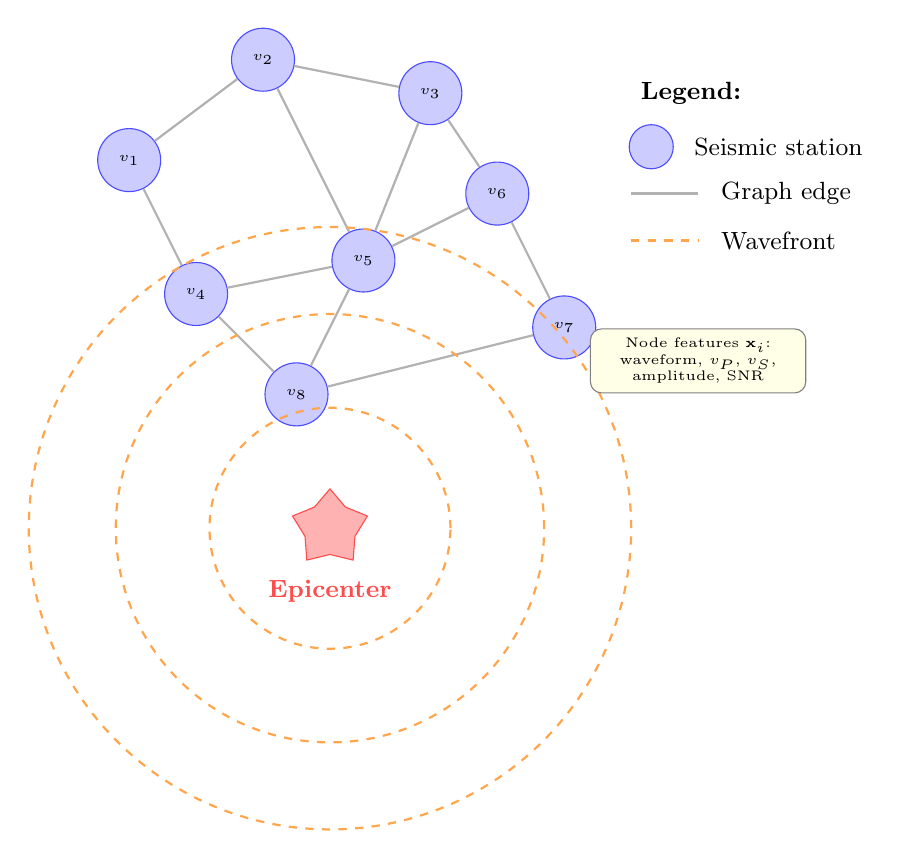
\begin{tikzpicture}[
  station/.style={circle, draw=blue!70, fill=blue!20, minimum size=8mm, inner sep=0pt, font=\tiny},
  epicenter/.style={star, star points=5, draw=red!70, fill=red!30, minimum size=10mm, inner sep=0pt},
  edge/.style={draw=gray!60, thick},
  wave/.style={draw=orange!70, dashed, thick},
  scale=0.85
]
  % Draw stations
  \node[station] (s1) at (0, 4) {$v_1$};
  \node[station] (s2) at (2, 5.5) {$v_2$};
  \node[station] (s3) at (4.5, 5) {$v_3$};
  \node[station] (s4) at (1, 2) {$v_4$};
  \node[station] (s5) at (3.5, 2.5) {$v_5$};
  \node[station] (s6) at (5.5, 3.5) {$v_6$};
  \node[station] (s7) at (6.5, 1.5) {$v_7$};
  \node[station] (s8) at (2.5, 0.5) {$v_8$};
  
  % Draw edges (connectivity)
  \draw[edge] (s1) -- (s2);
  \draw[edge] (s1) -- (s4);
  \draw[edge] (s2) -- (s3);
  \draw[edge] (s2) -- (s5);
  \draw[edge] (s3) -- (s6);
  \draw[edge] (s4) -- (s5);
  \draw[edge] (s4) -- (s8);
  \draw[edge] (s5) -- (s6);
  \draw[edge] (s5) -- (s8);
  \draw[edge] (s6) -- (s7);
  \draw[edge] (s7) -- (s8);
  \draw[edge] (s3) -- (s5);
  
  % Epicenter
  \node[epicenter] (eq) at (3, -1.5) {};
  \node[below=2mm of eq, font=\small\bfseries, red!70] {Epicenter};
  
  % Wavefronts
  \draw[wave] (eq) circle (1.8cm);
  \draw[wave] (eq) circle (3.2cm);
  \draw[wave] (eq) circle (4.5cm);
  
  % Labels
  \node[font=\small, anchor=west] at (7.5, 5) {\textbf{Legend:}};
  \node[station, scale=0.7] at (7.8, 4.2) {};
  \node[font=\small, anchor=west] at (8.3, 4.2) {Seismic station};
  \draw[edge] (7.5, 3.5) -- (8.5, 3.5);
  \node[font=\small, anchor=west] at (8.7, 3.5) {Graph edge};
  \draw[wave] (7.5, 2.8) -- (8.5, 2.8);
  \node[font=\small, anchor=west] at (8.7, 2.8) {Wavefront};
  
  % Node features annotation
  \node[draw=black!50, rounded corners, fill=yellow!10, font=\tiny, text width=2.5cm, align=center] at (8.5, 1) {Node features $\mathbf{x}_i$:\\waveform, $v_P$, $v_S$,\\amplitude, SNR};
\end{tikzpicture}
\caption{Illustration of a seismic monitoring network represented as a graph. Stations (nodes) are connected by edges encoding spatial relationships. Seismic wavefronts propagate outward from the earthquake epicenter, arriving at stations at different times depending on distance. The graph structure enables GNNs to model inter-station correlations and wavefield coherence.}
\label{fig:seismic_graph}
\end{figure}

\subsection{Graph Construction Strategies}

The choice of graph construction strategy---how to define the edge set $\mathcal{E}$ and associated edge weights---significantly influences GNN performance. Several approaches have been explored in the seismological context:

\textbf{Distance-based graphs}: The most common approach connects stations within a threshold distance $d_{\text{max}}$:
\begin{equation}
e_{ij} = \begin{cases} 1 & \text{if } \text{dist}(v_i, v_j) \leq d_{\text{max}} \\ 0 & \text{otherwise} \end{cases}
\end{equation}
Edge weights are typically computed using a Gaussian kernel: $w_{ij} = \exp(-\text{dist}(v_i, v_j)^2 / \sigma^2)$, where $\sigma$ controls the distance decay. This approach captures the physical intuition that nearby stations share similar ground motion characteristics, with the correlation decaying with distance \citep{vandenende2020automated, mcbrearty2023earthquake}.

\textbf{$k$-Nearest Neighbor ($k$-NN) graphs}: Each station is connected to its $k$ nearest neighbors, ensuring a minimum connectivity regardless of station density:
\begin{equation}
\mathcal{N}(v_i) = \text{arg top-}k_{v_j \in \mathcal{V} \setminus \{v_i\}} \left[ -\text{dist}(v_i, v_j) \right]
\end{equation}
This approach handles the heterogeneous station densities common in real networks, where urban areas may have stations separated by less than 10~km while rural regions have inter-station distances exceeding 100~km \citep{zhang2021spatiotemporal}.

\textbf{Voronoi tessellation-based graphs}: The Delaunay triangulation of station positions defines a natural planar graph that captures the geometric neighborhood structure. This approach produces edges that respect the spatial tessellation of the monitoring area and has been used in studies requiring physically interpretable connectivity \citep{yano2021graph}.

\textbf{Learned graph structures}: Rather than defining graph topology a priori, some approaches learn the adjacency matrix jointly with the GNN parameters. This allows the model to discover non-obvious station correlations---potentially reflecting shared geological structures, similar site conditions, or common noise sources---that may not correspond to geographic proximity \citep{bai2020adaptive, wu2020connecting}.

\subsection{Node and Edge Feature Engineering for Seismic Data}

The effectiveness of GNN-based seismic processing depends critically on the choice of node and edge features that encode relevant physical information.

\textbf{Node features} ($\mathbf{x}_i \in \mathbb{R}^F$) typically include:
\begin{itemize}
  \item Raw or preprocessed waveform segments (3-component: vertical, north, east)
  \item Spectral features: predominant period $\tau_c$, frequency content, spectral ratios
  \item Amplitude measures: peak displacement P$_d$, peak velocity, peak acceleration, cumulative absolute velocity (CAV)
  \item Temporal features: P-wave arrival time relative to origin time, time since first detection
  \item Station metadata: elevation, site classification ($V_{S30}$), instrument type, noise level
  \item Signal quality indicators: signal-to-noise ratio (SNR), data completeness
\end{itemize}

\textbf{Edge features} ($\mathbf{e}_{ij} \in \mathbb{R}^D$) encode pairwise station relationships:
\begin{itemize}
  \item Inter-station distance and azimuth
  \item Differential arrival times: $\Delta t_{ij} = t_i^P - t_j^P$
  \item Cross-correlation coefficients between waveforms at connected stations
  \item Geological path effects (velocity structure along the inter-station path)
  \item Relative site amplification factors
\end{itemize}

\subsection{Dynamic vs Static Graph Representations}

A critical design decision for GNN-based EEW is whether the graph structure should remain fixed (static) or evolve over time (dynamic).

\textbf{Static graphs} maintain a fixed adjacency matrix throughout processing, based on pre-computed station geometry. This approach is computationally efficient and suitable for tasks where the network configuration does not change during an event. Most existing work adopts static graphs \citep{vandenende2020automated, mcbrearty2023earthquake}.

\textbf{Dynamic graphs} allow the graph structure to evolve as an earthquake unfolds. As P-waves propagate outward from the source, stations are progressively ``activated'' (incorporated into the graph) as they detect signals. The graph at time $t$ includes only stations that have recorded arrivals:
\begin{equation}
\mathcal{V}(t) = \{v_i \in \mathcal{V} : t_i^{\text{detect}} \leq t\}
\end{equation}
This temporal evolution naturally captures the expanding spatial footprint of seismic observations and is particularly relevant for EEW, where decisions must be made with progressively increasing but initially sparse network observations \citep{munchmeyer2022team}. Dynamic graph approaches align with the sequential decision-making nature of EEW, where magnitude and location estimates are refined as additional stations report detections.

Hybrid approaches combine static backbone connectivity with dynamic node activation, maintaining edge definitions between all station pairs but only performing message passing through activated nodes. This formulation preserves computational efficiency while capturing the temporal evolution of network observations during an earthquake.


%% ============================================================
%% SECTION 4: GNN FUNDAMENTALS
%% ============================================================
\section{Graph Neural Network Fundamentals}
\label{sec:gnn_fundamentals}

\subsection{Message Passing Framework}

The unifying computational paradigm underlying most modern GNN architectures is the message passing neural network (MPNN) framework \citep{gilmer2017neural}, which generalizes earlier gated graph sequence models \citep{li2016gated}. In this framework, each node iteratively updates its representation by aggregating information from its neighbors through a sequence of message passing layers. A theoretical analysis of the expressive power of such architectures, connecting them to the Weisfeiler-Leman graph isomorphism test, is provided by \citet{morris2019weisfeiler} and \citet{xu2019powerful}. For a node $v_i$ with hidden representation $\mathbf{h}_i^{(l)}$ at layer $l$, the update is:

\begin{align}
\mathbf{m}_i^{(l+1)} &= \bigoplus_{j \in \mathcal{N}(i)} \phi\left(\mathbf{h}_i^{(l)}, \mathbf{h}_j^{(l)}, \mathbf{e}_{ij}\right) \label{eq:message} \\
\mathbf{h}_i^{(l+1)} &= \psi\left(\mathbf{h}_i^{(l)}, \mathbf{m}_i^{(l+1)}\right) \label{eq:update}
\end{align}

where $\phi$ is the message function computing interactions between connected nodes, $\bigoplus$ is a permutation-invariant aggregation operator (sum, mean, or max), and $\psi$ is the update function that combines the aggregated messages with the node's current state. The initial node representations are $\mathbf{h}_i^{(0)} = \mathbf{x}_i$.

After $L$ layers of message passing, each node's representation $\mathbf{h}_i^{(L)}$ encodes information from its $L$-hop neighborhood---the set of all nodes reachable within $L$ graph traversal steps. For EEW applications, this receptive field determines how far across the seismic network information can propagate, with implications for the model's ability to capture network-wide wavefield patterns.

For graph-level predictions (e.g., earthquake magnitude from the entire network), a readout function aggregates all node representations:
\begin{equation}
\mathbf{h}_{\mathcal{G}} = \text{READOUT}\left(\{\mathbf{h}_i^{(L)} : v_i \in \mathcal{V}\}\right)
\end{equation}

\subsection{Spectral Methods}

Spectral graph neural networks define convolution operations through the graph Fourier transform, leveraging the eigendecomposition of the graph Laplacian matrix $\mathbf{L} = \mathbf{D} - \mathbf{A}$, where $\mathbf{D}$ is the degree matrix and $\mathbf{A}$ is the adjacency matrix.

\textbf{ChebNet} \citep{defferrard2016convolutional} approximates spectral graph convolutions using Chebyshev polynomials $T_k$ of the normalized Laplacian $\tilde{\mathbf{L}} = 2\mathbf{L}/\lambda_{\max} - \mathbf{I}$:
\begin{equation}
\mathbf{h}_i^{(l+1)} = \sigma\left(\sum_{k=0}^{K-1} \theta_k T_k(\tilde{\mathbf{L}}) \mathbf{h}_i^{(l)}\right)
\end{equation}
where $K$ determines the polynomial order (localization radius) and $\theta_k$ are learnable parameters. This formulation enables localized filtering without computing the full eigendecomposition, achieving $O(K|\mathcal{E}|)$ complexity.

\textbf{Graph Convolutional Network (GCN)} \citep{kipf2017semi} simplifies ChebNet by using first-order approximation ($K=1$) with renormalization:
\begin{equation}
\mathbf{H}^{(l+1)} = \sigma\left(\tilde{\mathbf{D}}^{-1/2}\tilde{\mathbf{A}}\tilde{\mathbf{D}}^{-1/2}\mathbf{H}^{(l)}\mathbf{W}^{(l)}\right)
\end{equation}
where $\tilde{\mathbf{A}} = \mathbf{A} + \mathbf{I}$ includes self-loops, $\tilde{\mathbf{D}}_{ii} = \sum_j \tilde{\mathbf{A}}_{ij}$, and $\mathbf{W}^{(l)}$ is a learnable weight matrix. GCN has become the most widely adopted baseline architecture for graph learning tasks, including initial explorations in seismology \citep{bilal2022graph, bloemheuvel2022graph}.

For seismic applications, spectral methods offer the advantage of well-understood frequency-domain properties but are limited to fixed graph topologies (the Laplacian eigendecomposition is graph-specific), which restricts their applicability to dynamic network scenarios.

\subsection{Spatial Methods}

Spatial GNN methods define convolution directly in the vertex domain, operating through neighborhood aggregation without requiring spectral decomposition.

\textbf{GraphSAGE} \citep{hamilton2017inductive} introduces sampling-based neighborhood aggregation for inductive learning:
\begin{align}
\mathbf{h}_{\mathcal{N}(i)}^{(l)} &= \text{AGG}\left(\{\mathbf{h}_j^{(l-1)} : j \in \mathcal{N}(i)\}\right) \\
\mathbf{h}_i^{(l)} &= \sigma\left(\mathbf{W}^{(l)} \cdot \left[\mathbf{h}_i^{(l-1)} \| \mathbf{h}_{\mathcal{N}(i)}^{(l)}\right]\right)
\end{align}
where AGG is an aggregation function (mean, LSTM, or max-pooling) and $\|$ denotes concatenation. GraphSAGE's inductive capability---learning generalizable aggregation functions rather than node-specific embeddings---is particularly valuable for seismology, where models trained on one network region must generalize to other regions with different station configurations.

\textbf{Graph Attention Network (GAT)} \citep{velickovic2018graph} introduces attention mechanisms to learn adaptive weighting of neighbor contributions:
\begin{equation}
\alpha_{ij} = \frac{\exp\left(\text{LeakyReLU}\left(\mathbf{a}^T[\mathbf{W}\mathbf{h}_i \| \mathbf{W}\mathbf{h}_j]\right)\right)}{\sum_{k \in \mathcal{N}(i)} \exp\left(\text{LeakyReLU}\left(\mathbf{a}^T[\mathbf{W}\mathbf{h}_i \| \mathbf{W}\mathbf{h}_k]\right)\right)}
\end{equation}
\begin{equation}
\mathbf{h}_i^{(l+1)} = \sigma\left(\sum_{j \in \mathcal{N}(i)} \alpha_{ij} \mathbf{W}\mathbf{h}_j^{(l)}\right)
\end{equation}

Multi-head attention extends this by concatenating $H$ independent attention heads. For EEW, the attention mechanism provides physically interpretable weights: stations contributing more informative signals (higher SNR, closer to the epicenter, better azimuthal coverage) naturally receive higher attention weights, and these weights can be visualized to understand model decision-making \citep{vandenende2020automated}.

\textbf{Graph Isomorphism Network (GIN)} \citep{xu2019powerful} achieves maximal expressiveness among message-passing GNNs by using summation aggregation with a learnable parameter $\epsilon$:
\begin{equation}
\mathbf{h}_i^{(l+1)} = \text{MLP}^{(l)}\left((1 + \epsilon^{(l)}) \cdot \mathbf{h}_i^{(l)} + \sum_{j \in \mathcal{N}(i)} \mathbf{h}_j^{(l)}\right)
\end{equation}
GIN's theoretical expressiveness makes it suitable for tasks requiring fine discrimination between different graph structures---relevant when distinguishing seismic events with subtly different source characteristics observed through similar network geometries.

\subsection{Temporal Graph Networks}

Seismic data is inherently temporal, requiring architectures that jointly capture spatial (inter-station) and temporal (within-waveform) patterns.

\textbf{T-GCN} \citep{zhao2020tgcn} combines Graph Convolutional layers for spatial processing with Gated Recurrent Units (GRUs) for temporal modeling:
\begin{align}
\mathbf{f}^{(t)} &= \text{GCN}\left(\mathbf{X}^{(t)}, \mathbf{A}\right) \\
\mathbf{h}^{(t)} &= \text{GRU}\left(\mathbf{f}^{(t)}, \mathbf{h}^{(t-1)}\right)
\end{align}
This architecture processes spatial correlations at each time step, then captures temporal dynamics through the recurrent mechanism.

\textbf{A3T-GCN} extends T-GCN with attention mechanisms that adaptively weight temporal observations, allowing the model to focus on the most informative time steps---such as the initial P-wave onset or the transition to S-wave arrival \citep{bai2020adaptive}.

\textbf{DCRNN} (Diffusion Convolutional Recurrent Neural Network) \citep{li2018dcrnn} models spatial dependencies through bidirectional random walks on the graph, integrated with sequence-to-sequence learning for temporal prediction:
\begin{equation}
\mathbf{H}^{(l)} = \sum_{k=0}^{K} \left(\theta_{k,1} \left(\mathbf{D}_O^{-1}\mathbf{A}\right)^k + \theta_{k,2} \left(\mathbf{D}_I^{-1}\mathbf{A}^T\right)^k\right) \mathbf{X}
\end{equation}
where $\mathbf{D}_O$ and $\mathbf{D}_I$ are the out-degree and in-degree matrices. The diffusion process naturally captures wave propagation patterns on the station graph.

\textbf{Spatio-Temporal Graph Convolutional Networks (STGCN)} \citep{yu2018spatio} interleave temporal convolution (1D causal convolutions along the time axis) with spatial graph convolution, avoiding the sequential processing bottleneck of RNN-based approaches while maintaining receptive field growth through dilated convolutions.

\subsection{Graph Transformers}

Recent work has extended the Transformer architecture \citep{vaswani2017attention} to graph-structured data, combining the expressiveness of global self-attention with structural graph information.

\textbf{Graphormer} \citep{ying2021transformers} incorporates graph structure through spatial encodings (shortest-path distances), edge encodings (features along shortest paths), and centrality encodings (node degree information) into the standard Transformer attention mechanism. This allows attention to be computed between all node pairs while remaining sensitive to graph topology.

\textbf{Graph Transformer} architectures \citep{dwivedi2021generalization} adapt positional encodings for graphs using Laplacian eigenvectors or random walk probabilities as positional features. For seismic networks, these positional encodings can capture the geometric arrangement of stations relative to potential source locations.

Graph Transformers offer the advantage of global receptive fields (every node can attend to every other node) without the depth limitations of message-passing networks, which may be beneficial for large-scale seismic networks where wavefield information must propagate across many hops.

\subsection{Pooling and Readout Operations}

For graph-level predictions in EEW (e.g., estimating a single magnitude value from the entire network), node representations must be aggregated into a fixed-size graph representation.

\textbf{Global pooling} operations (sum, mean, max) provide simple permutation-invariant aggregation:
\begin{equation}
\mathbf{h}_{\mathcal{G}} = \frac{1}{|\mathcal{V}|} \sum_{i \in \mathcal{V}} \mathbf{h}_i^{(L)}
\end{equation}

\textbf{Hierarchical pooling} methods \citep{ying2018hierarchical} learn to progressively coarsen the graph, identifying clusters of stations that can be summarized together---potentially discovering meaningful spatial groupings (e.g., stations on similar geological units, stations at similar epicentral distances).

\textbf{Attention-based pooling} \citep{lee2019self} computes importance scores for each node and performs weighted aggregation, effectively learning which stations are most informative for a given prediction task. In EEW, stations closer to the epicenter with clear P-wave onsets would naturally receive higher attention weights.

\begin{figure}[htbp]
\centering
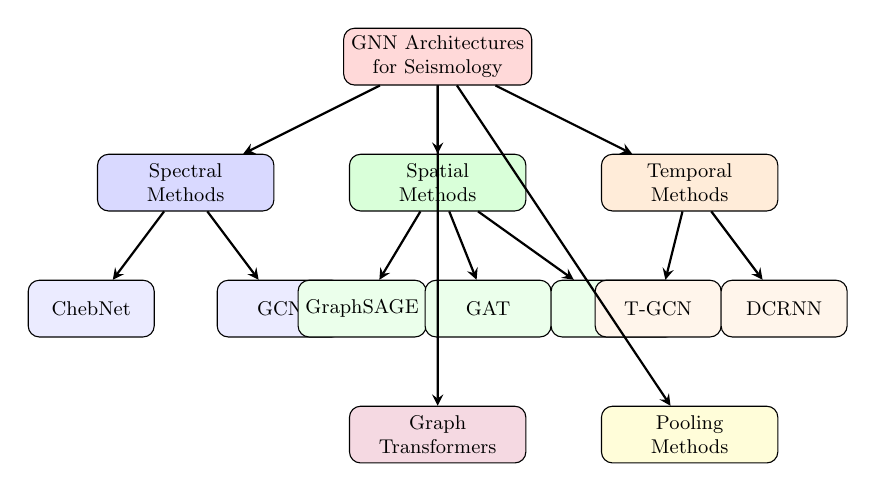
\begin{tikzpicture}[
  box/.style={draw, rounded corners, minimum width=2.8cm, minimum height=0.9cm, align=center, font=\small},
  arrow/.style={->, thick, >=stealth},
  level/.style={font=\small\bfseries},
  scale=0.8, transform shape
]
  % Root
  \node[box, fill=red!15] (root) at (5, 8) {GNN Architectures\\for Seismology};
  
  % Level 1
  \node[box, fill=blue!15] (spectral) at (1, 6) {Spectral\\Methods};
  \node[box, fill=green!15] (spatial) at (5, 6) {Spatial\\Methods};
  \node[box, fill=orange!15] (temporal) at (9, 6) {Temporal\\Methods};
  
  % Level 2 - Spectral
  \node[box, fill=blue!8, minimum width=2cm] (cheb) at (-0.5, 4) {ChebNet};
  \node[box, fill=blue!8, minimum width=2cm] (gcn) at (2.5, 4) {GCN};
  
  % Level 2 - Spatial
  \node[box, fill=green!8, minimum width=2cm] (sage) at (3.8, 4) {GraphSAGE};
  \node[box, fill=green!8, minimum width=2cm] (gat) at (5.8, 4) {GAT};
  \node[box, fill=green!8, minimum width=2cm] (gin) at (7.8, 4) {GIN};
  
  % Level 2 - Temporal
  \node[box, fill=orange!8, minimum width=2cm] (tgcn) at (8.5, 4) {T-GCN};
  \node[box, fill=orange!8, minimum width=2cm] (dcrnn) at (10.5, 4) {DCRNN};
  
  % Advanced
  \node[box, fill=purple!15] (transformer) at (5, 2) {Graph\\Transformers};
  \node[box, fill=yellow!15] (pool) at (9, 2) {Pooling\\Methods};
  
  % Arrows
  \draw[arrow] (root) -- (spectral);
  \draw[arrow] (root) -- (spatial);
  \draw[arrow] (root) -- (temporal);
  \draw[arrow] (spectral) -- (cheb);
  \draw[arrow] (spectral) -- (gcn);
  \draw[arrow] (spatial) -- (sage);
  \draw[arrow] (spatial) -- (gat);
  \draw[arrow] (spatial) -- (gin);
  \draw[arrow] (temporal) -- (tgcn);
  \draw[arrow] (temporal) -- (dcrnn);
  \draw[arrow] (root) -- (transformer);
  \draw[arrow] (root) -- (pool);
\end{tikzpicture}
\caption{Taxonomy of Graph Neural Network architectures applicable to seismological data processing. Methods are categorized into spectral approaches (operating in the graph frequency domain), spatial approaches (aggregating in the vertex domain), temporal approaches (combining spatial and temporal modeling), graph transformers (global attention with structural encoding), and pooling methods (graph-level representation learning).}
\label{fig:gnn_taxonomy}
\end{figure}


%% ============================================================
%% SECTION 5: GNN APPLICATIONS IN SEISMOLOGY
%% ============================================================
\section{GNN Applications in Seismology}
\label{sec:applications}

\subsection{Seismic Phase Picking and Event Detection}

Phase picking---the identification of P-wave and S-wave arrival times on seismograms---constitutes the foundational task in seismic data processing. Accurate phase picks are prerequisites for earthquake location, magnitude estimation, and tomographic imaging. Traditional methods including STA/LTA ratio algorithms \citep{allen1978automatic, withers1998comparison} and manual analyst picks, while well-established, face limitations in throughput, consistency, and performance in low-SNR environments.

The application of GNNs to phase picking represents a paradigm shift from station-independent processing to network-aware detection. \citet{bilal2022graph} demonstrated that GNN-based phase detection incorporating multi-station spatial correlations achieves superior performance compared to single-station CNN methods, particularly for small-magnitude events where individual station recordings may be ambiguous. Their approach constructs a graph over the seismic network and applies GAT layers to aggregate spatial context, enabling the model to leverage correlated arrivals at multiple stations for more confident phase identification.

\citet{munchmeyer2021gnn} applied GNNs to the closely related task of phase association---determining which detected phases belong to the same seismic event. This combinatorial problem, which scales quadratically with the number of detections in traditional grid-search methods, is naturally formulated as edge classification on a detection graph where nodes represent phase picks and edges connect potentially associated picks. The GNN learns to predict edge labels (same-event or different-event) by aggregating features from neighboring picks, achieving significant improvements in association accuracy for complex sequences with overlapping events. Earlier deep learning approaches to phase association include PhaseLink \citep{ross2019phaselink}, while Bayesian methods such as GAMMA \citep{zhu2022earthquake} provide complementary probabilistic frameworks. Scalable workflow systems such as QuakeFlow \citep{johnson2021quakeflow} integrate these association methods into end-to-end monitoring pipelines.

\citet{bloemheuvel2022graph} proposed a graph-based framework for seismic phase classification that jointly models spatial and temporal relationships between waveform segments across the network. By operating on graphs where nodes carry short waveform windows and edges encode spatial proximity, the model achieves robust classification even in scenarios with multiple simultaneous events or high cultural noise levels.

\subsection{Earthquake Source Characterization}

Earthquake source characterization encompasses the estimation of source parameters including hypocenter location, focal mechanism (fault orientation and slip direction), rupture geometry, and stress drop. \citet{vandenende2020automated} presented one of the earliest applications of deep GNNs to seismic source characterization, demonstrating that a GNN operating on the station network graph can directly estimate moment tensor components from multi-station waveform recordings. Their architecture processes three-component waveforms at each station through CNN feature extractors, then aggregates across stations using graph neural network layers, producing a single moment tensor estimate for the network. The approach showed particular advantages for events recorded by sparse networks, where the spatial reasoning enabled by the GNN compensates for limited azimuthal coverage.

\citet{zhang2021spatiotemporal} extended this work with spatiotemporal graph convolutional networks that jointly model the time-evolving wavefield across the station network. Their architecture interleaves temporal convolutions (capturing waveform evolution at each station) with spatial graph convolutions (aggregating across stations), achieving improved characterization of complex ruptures where the source time function evolves over multiple seconds. Further developments include deep deconvolution methods for source characterization using GNNs \citep{vandenende2022deep}, graph-based seismic event classification frameworks \citep{zhang2022graph}, and graph neural networks applied to multivariate seismic time series \citep{bloemheuvel2022graph}.

\subsection{Magnitude Estimation}

Rapid magnitude estimation from initial P-wave seconds represents one of the most critical EEW tasks, as magnitude directly determines predicted ground motion intensity and thus alert decisions. Traditional approaches using empirical scaling relationships between initial waveform parameters ($\tau_c$, P$_d$) and final magnitude suffer from well-documented saturation effects for large events.

\citet{mcbrearty2023earthquake} demonstrated that GNNs can estimate earthquake magnitude with significantly reduced uncertainty compared to single-station methods by leveraging multi-station P-wave observations through graph-based processing. Their approach achieves magnitude estimates within 0.2--0.3 units of catalog values using only 4--8 seconds of data following the first P-wave arrival, representing a substantial improvement over the 0.5--1.0 unit uncertainties typical of traditional methods.

\citet{jozinovic2022transfer} applied transfer learning with graph neural networks to ground motion prediction, demonstrating that GNN-based models trained on data-rich regions can be effectively adapted to data-sparse regions, achieving robust performance even when target-domain training data is limited to a few hundred recordings.

\subsection{Ground Motion Prediction}

Predicting ground motion intensity (Peak Ground Acceleration, Peak Ground Velocity, spectral accelerations) at target sites distant from the epicenter is the ultimate goal of EEW systems. Traditional Ground Motion Prediction Equations (GMPEs) \citep{abrahamson2014nga, boore2014nga} provide expected ground motion as functions of magnitude, distance, and site conditions, but exhibit large aleatory variability (scatter around median predictions) and poorly capture spatial correlations in ground motion fields.

\citet{jozinovic2022ground} applied GNNs to ground motion prediction, treating the target prediction sites and recording stations jointly as nodes in a graph. The GNN learns to interpolate and extrapolate ground motion fields by aggregating observations from recorded stations to predict values at unobserved target locations, naturally capturing the spatial correlations that GMPEs ignore. Their model reduces prediction residuals by 20--30\% compared to standard GMPEs for scenarios with moderate station coverage.

\citet{ni2023graph} developed a graph neural network for site-specific ground motion prediction that incorporates geological features (basin depth, $V_{S30}$, sediment thickness) as node attributes and fault geometry information as edge features. The approach demonstrates that GNNs can effectively combine path effects, site effects, and source effects in a unified framework that outperforms conventional empirical models.

\subsection{Seismic Source Location}

Earthquake location---determining the hypocenter (latitude, longitude, depth) from observed arrival times---is classically solved through iterative nonlinear inversion. GNN-based approaches reformulate location as a regression or classification task on the station network graph.

\citet{mcbrearty2023earthquake} showed that GNN location estimates achieve median errors of 2--5~km using P-wave arrival times from 5--10 stations, competitive with traditional methods while providing faster inference suitable for real-time EEW. The model learns implicit velocity structure from training data, avoiding the need for explicit 1-D or 3-D velocity models that introduce systematic biases.

Graph-based location methods offer particular advantages for: (1) events near the edge of networks where ray coverage is limited; (2) induced seismicity monitoring where precise locations require dense local arrays; and (3) real-time applications where iterative inversion may be too slow. The permutation-invariant nature of GNNs ensures robustness to varying numbers of detecting stations, a common situation in operational EEW where not all network stations detect every event.

\subsection{Aftershock Prediction}

Aftershock forecasting---predicting the spatial, temporal, and magnitude distribution of future earthquakes following a mainshock---represents an increasingly important application of data-driven methods. \citet{devries2018deep} demonstrated that deep learning approaches can outperform Coulomb stress models for spatial aftershock prediction (though the simplicity of effective models has been debated \citep{mignan2020one}), motivating graph-based extensions. Machine learning has also been applied to laboratory earthquake prediction \citep{rouetleduc2017machine, johnson2021laboratory}, establishing that data-driven methods can capture precursory signals in fault systems.

GNN architectures for aftershock prediction represent the fault network as a graph, where nodes correspond to discretized fault patches and edges encode stress transfer relationships. The graph formulation naturally captures the complex geometry of fault systems and the long-range stress interactions that drive aftershock sequences. Recent work combines GNNs with physics-informed constraints derived from elastic dislocation theory to produce physically plausible predictions \citep{wang2021injection}.

\subsection{Induced Seismicity Monitoring}

Induced seismicity from fluid injection (wastewater disposal, hydraulic fracturing, enhanced geothermal systems) has emerged as a significant concern, requiring real-time monitoring systems capable of detecting and characterizing small-magnitude events in noisy environments \citep{ellsworth2013injection}. GNN-based approaches have been developed for induced seismicity detection that leverage the dense local monitoring networks typically deployed around injection sites.

The graph representation is particularly natural for induced seismicity arrays, where station separations are small (hundreds of meters to a few kilometers) and coherent signals are expected across multiple stations even for microseismic events (M$<$0). \citet{wang2021injection} applied graph-based architectures for induced seismicity forecasting, using the spatial-temporal evolution of seismicity as input features on a graph representing the injection field.

\begin{table}[htbp]
\centering
\caption{Comparison of GNN methods for different seismic tasks. Performance metrics are drawn from the cited publications.}
\label{tab:gnn_comparison}
\small
\begin{tabular}{p{2.5cm}p{2.5cm}p{2.5cm}p{2cm}p{2.5cm}}
\toprule
\textbf{Method} & \textbf{Architecture} & \textbf{Task} & \textbf{Dataset} & \textbf{Performance} \\
\midrule
\citet{vandenende2020automated} & GCN + CNN & Source characterization & SoCal synthetic & Moment tensor RMSE: 0.12 \\
\citet{zhang2021spatiotemporal} & ST-GCN & Source characterization & SCEDC & Location error: 3.2~km \\
\citet{mcbrearty2023earthquake} & GAT + MLP & Location + magnitude & NorCal & Mag MAE: 0.21, Loc: 2.8~km \\
\citet{bilal2022graph} & GCN & Phase detection & STEAD & F1: 0.94 (P), 0.91 (S) \\
\citet{munchmeyer2021gnn} & Edge GNN & Phase association & INSTANCE & Precision: 0.96 \\
\citet{ni2023graph} & GAT & Ground motion & Japan K-NET & $\sigma$ reduction: approx.\ 25\% \\
\citet{jozinovic2022transfer} & GNN + Transfer & Ground motion & Multi-region & RMSE reduction: approx.\ 20\% \\
\citet{munchmeyer2022team} & Transformer GNN & EEW magnitude & Multi-station & Alert time: $<$5s avg \\
\bottomrule
\end{tabular}
\end{table}

\begin{figure}[htbp]
\centering
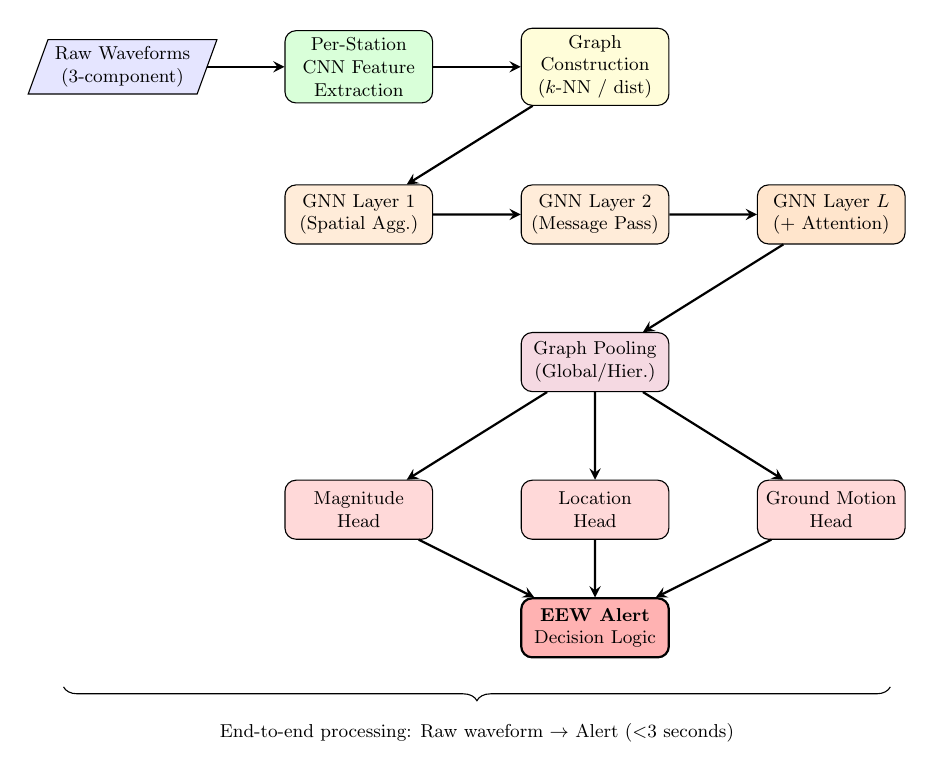
\begin{tikzpicture}[
  block/.style={draw, rounded corners, minimum width=2.5cm, minimum height=1cm, align=center, font=\small},
  arrow/.style={->, thick, >=stealth},
  data/.style={draw, trapezium, trapezium left angle=70, trapezium right angle=110, minimum width=2cm, minimum height=0.7cm, align=center, font=\small},
  scale=0.75, transform shape
]
  % Input layer
  \node[data, fill=blue!10] (raw) at (0, 0) {Raw Waveforms\\(3-component)};
  
  % Feature extraction
  \node[block, fill=green!15] (cnn) at (4, 0) {Per-Station\\CNN Feature\\Extraction};
  
  % Graph construction
  \node[block, fill=yellow!15] (graph) at (8, 0) {Graph\\Construction\\($k$-NN / dist)};
  
  % GNN processing
  \node[block, fill=orange!15] (gnn1) at (4, -2.5) {GNN Layer 1\\(Spatial Agg.)};
  \node[block, fill=orange!15] (gnn2) at (8, -2.5) {GNN Layer 2\\(Message Pass)};
  \node[block, fill=orange!20] (gnn3) at (12, -2.5) {GNN Layer $L$\\(+ Attention)};
  
  % Pooling
  \node[block, fill=purple!15] (pool) at (8, -5) {Graph Pooling\\(Global/Hier.)};
  
  % Output heads
  \node[block, fill=red!15] (mag) at (4, -7.5) {Magnitude\\Head};
  \node[block, fill=red!15] (loc) at (8, -7.5) {Location\\Head};
  \node[block, fill=red!15] (gm) at (12, -7.5) {Ground Motion\\Head};
  
  % Alert
  \node[block, fill=red!30, thick] (alert) at (8, -9.5) {\textbf{EEW Alert}\\Decision Logic};
  
  % Arrows
  \draw[arrow] (raw) -- (cnn);
  \draw[arrow] (cnn) -- (graph);
  \draw[arrow] (graph) -- (gnn1);
  \draw[arrow] (gnn1) -- (gnn2);
  \draw[arrow] (gnn2) -- (gnn3);
  \draw[arrow] (gnn3) -- (pool);
  \draw[arrow] (pool) -- (mag);
  \draw[arrow] (pool) -- (loc);
  \draw[arrow] (pool) -- (gm);
  \draw[arrow] (mag) -- (alert);
  \draw[arrow] (loc) -- (alert);
  \draw[arrow] (gm) -- (alert);
  
  % Time annotation
  \draw[decorate, decoration={brace, amplitude=5pt, mirror}] (-1, -10.5) -- (13, -10.5);
  \node[font=\small, below] at (6, -11) {End-to-end processing: Raw waveform $\rightarrow$ Alert ($<$3 seconds)};
\end{tikzpicture}
\caption{Architecture of a GNN-based Earthquake Early Warning pipeline. Raw three-component waveforms undergo per-station CNN feature extraction, are assembled into a graph based on network topology, processed through multiple GNN layers with message passing and attention, pooled into graph-level representations, and passed to task-specific heads for magnitude, location, and ground motion estimation. Alert decisions integrate all predictions.}
\label{fig:eew_pipeline}
\end{figure}


%% ============================================================
%% SECTION 6: TEMPORAL-SPATIAL GRAPH NETWORKS
%% ============================================================
\section{Temporal-Spatial Graph Networks for Seismic Data}
\label{sec:temporal_spatial}

\subsection{Spatio-temporal Feature Extraction}

Seismic data presents a unique spatio-temporal processing challenge: waveforms recorded at each station contain rich temporal structure (P-wave onset, S-wave coda, frequency content evolution), while the spatial distribution of recordings across the network encodes source location and propagation effects. Effective GNN architectures for EEW must jointly capture both dimensions.

The spatio-temporal feature extraction paradigm typically follows one of three design patterns:

\textbf{Sequential spatial-then-temporal}: Spatial graph convolutions aggregate multi-station features at each time step, producing spatially-aware node representations that are subsequently processed through temporal models (LSTM, GRU, or temporal convolutions). This approach, adopted by T-GCN \citep{zhao2020tgcn} and its variants, first builds a spatial context for each station, then models how this context evolves over time.

\textbf{Interleaved spatial-temporal}: Alternating spatial and temporal processing layers progressively build joint representations. STGCN \citep{yu2018spatio} interleaves temporal convolution blocks (1D convolutions along time) with spatial graph convolution blocks, allowing spatial and temporal patterns to interact at multiple scales. For seismic data, this enables the model to learn, for example, that P-wave arrivals at nearby stations create characteristic spatio-temporal patterns that differ from noise.

\textbf{Unified spatio-temporal}: Some architectures define convolutions on spatio-temporal graphs where nodes represent station-time pairs and edges connect both spatially adjacent stations and temporally adjacent time steps at the same station. This creates a higher-dimensional graph that captures both relationships simultaneously but at increased computational cost.

For EEW applications, the choice of architecture must balance representation power against inference speed. The interleaved approach offers a favorable trade-off, enabling progressive refinement of spatio-temporal features while maintaining manageable computational requirements through efficient 1D temporal convolutions and sparse graph operations.

\subsection{Attention Mechanisms for Seismic Graphs}

Attention mechanisms \citep{bahdanau2015neural} play a crucial role in GNN-based seismic processing by enabling adaptive weighting of both spatial (inter-station) and temporal (intra-waveform) information.

\textbf{Spatial attention}: In the context of EEW, not all stations contribute equally to source characterization. Stations closer to the epicenter provide the most direct constraint on location and magnitude, while stations with higher noise levels or sensor issues should be down-weighted. GAT-style attention \citep{velickovic2018graph} naturally learns these weightings from data:
\begin{equation}
\alpha_{ij}^{(l)} = \text{softmax}_j\left(\frac{(\mathbf{W}_Q\mathbf{h}_i^{(l)})^T (\mathbf{W}_K\mathbf{h}_j^{(l)})}{\sqrt{d_k}}\right)
\end{equation}
where the query $\mathbf{W}_Q\mathbf{h}_i$ from the target station learns to attend selectively to keys $\mathbf{W}_K\mathbf{h}_j$ from neighboring stations based on their current feature representations.

\textbf{Temporal attention}: Within each station's waveform, different time windows contain varying amounts of information. The initial P-wave onset is maximally informative for arrival time determination, while slightly later windows may better constrain magnitude through amplitude growth patterns. Temporal attention mechanisms \citep{guo2019attention} learn to focus on the most diagnostic portions of each waveform:
\begin{equation}
\beta_t = \text{softmax}\left(\mathbf{v}^T \tanh(\mathbf{W}_t\mathbf{h}^{(t)} + \mathbf{b}_t)\right)
\end{equation}
where $\beta_t$ is the attention weight for time step $t$.

\textbf{Cross-attention}: Some architectures implement cross-attention between spatial and temporal dimensions, allowing the model to learn correlations such as ``focus on later time windows at more distant stations'' (because P-waves arrive later) or ``weight early arrivals more heavily at the closest stations'' (because these provide the first constraint on source parameters).

\subsection{Multi-scale Temporal Modeling}

Seismic events exhibit characteristic temporal patterns at multiple scales: millisecond-scale high-frequency onsets, second-scale waveform envelopes, and multi-second source duration effects for large earthquakes. Effective GNN architectures must capture these multi-scale temporal features.

\textbf{Dilated temporal convolutions} expand the receptive field exponentially with depth while maintaining resolution at each scale. For seismic data sampled at 100~Hz, a cascade of dilated convolutions with dilation factors [1, 2, 4, 8, 16] covers temporal scales from 10~ms to 160~ms at the first level, expandable to seconds through stacking.

\textbf{Multi-resolution temporal encoding}: Parallel temporal processing at different sampling rates captures both high-frequency onset characteristics and lower-frequency envelope features. The outputs from each resolution are concatenated or fused through attention before spatial graph processing.

\textbf{Wavelet-based features}: Computing continuous wavelet transforms (CWT) provides time-frequency representations that can serve as rich node features, encoding both the spectral content and its temporal evolution. These features have proven particularly effective for magnitude estimation, where the frequency content of initial P-waves correlates with final magnitude through source scaling relationships. Differentiable time-series alignment methods such as soft-DTW \citep{cuturi2017soft} can further enhance temporal feature extraction by enabling learned alignment of waveforms across stations.

\subsection{Dynamic Graph Learning for Evolving Networks}

The sequential nature of P-wave propagation across a seismic network creates a naturally dynamic graph structure. As time progresses from the earthquake origin:

\begin{enumerate}
  \item At $t = t_0$: Only the closest station(s) detect P-waves; the graph has 1--2 active nodes
  \item At $t = t_0 + 2$s: P-waves reach additional nearby stations; 3--8 active nodes
  \item At $t = t_0 + 5$s: P-waves propagate to more distant stations; 10--20+ active nodes
  \item At $t = t_0 + 10$s: Most regional stations activated; near-full network observations
\end{enumerate}

Dynamic graph learning architectures that explicitly model this progressive activation achieve superior EEW performance because they can:
\begin{itemize}
  \item Issue preliminary estimates with minimal stations (fast but uncertain)
  \item Progressively refine estimates as additional stations report (accuracy improves with time)
  \item Naturally handle varying network sizes and station outages
  \item Model the information gain from each newly activated station
\end{itemize}

\citet{munchmeyer2022team} proposed the Transformer Earthquake Alerting Model (TEAM) for EEW that implements multi-station waveform processing, treating the seismic network as a graph and outputting updated source parameter estimates with progressively increasing station counts. Their model achieves operational-quality estimates within 4--6 seconds of the first P-wave detection, with uncertainty monotonically decreasing as additional stations contribute observations.

\begin{figure}[htbp]
\centering
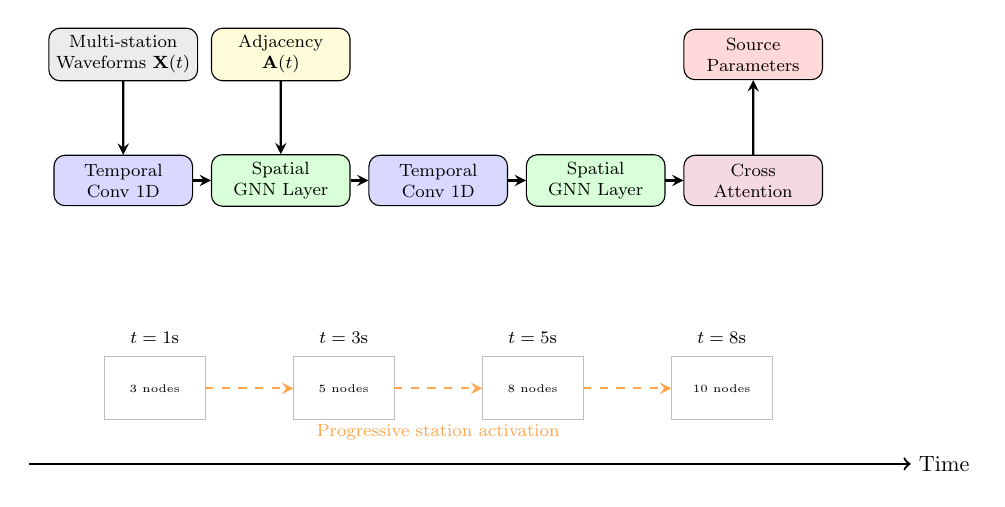
\begin{tikzpicture}[
  block/.style={draw, rounded corners, minimum width=2.2cm, minimum height=0.8cm, align=center, font=\footnotesize},
  arrow/.style={->, thick, >=stealth},
  dashedarrow/.style={->, dashed, thick, >=stealth},
  scale=0.8, transform shape
]
  % Time axis
  \draw[->, thick] (0, -4.5) -- (14, -4.5) node[right] {Time};
  
  % Temporal blocks
  \node[block, fill=blue!15] (t1) at (1.5, 0) {Temporal\\Conv 1D};
  \node[block, fill=green!15] (s1) at (4, 0) {Spatial\\GNN Layer};
  \node[block, fill=blue!15] (t2) at (6.5, 0) {Temporal\\Conv 1D};
  \node[block, fill=green!15] (s2) at (9, 0) {Spatial\\GNN Layer};
  \node[block, fill=purple!15] (att) at (11.5, 0) {Cross\\Attention};
  
  % Input
  \node[block, fill=gray!15] (input) at (1.5, 2) {Multi-station\\Waveforms $\mathbf{X}(t)$};
  
  % Graph structure
  \node[block, fill=yellow!15] (adj) at (4, 2) {Adjacency\\$\mathbf{A}(t)$};
  
  % Output
  \node[block, fill=red!15] (out) at (11.5, 2) {Source\\Parameters};
  
  % Arrows
  \draw[arrow] (input) -- (t1);
  \draw[arrow] (t1) -- (s1);
  \draw[arrow] (adj) -- (s1);
  \draw[arrow] (s1) -- (t2);
  \draw[arrow] (t2) -- (s2);
  \draw[arrow] (s2) -- (att);
  \draw[arrow] (att) -- (out);
  
  % Dynamic graph illustration
  \node[font=\footnotesize] at (2, -2.5) {$t=1$s};
  \node[font=\footnotesize] at (5, -2.5) {$t=3$s};
  \node[font=\footnotesize] at (8, -2.5) {$t=5$s};
  \node[font=\footnotesize] at (11, -2.5) {$t=8$s};
  
  % Small graph visualizations
  \foreach \x/\n in {2/3, 5/5, 8/8, 11/10} {
    \draw[gray!50] (\x-0.8, -3.8) rectangle (\x+0.8, -2.8);
    \node[font=\tiny] at (\x, -3.3) {\n~nodes};
  }
  
  % Progressive arrow
  \draw[dashedarrow, orange!70] (2.8, -3.3) -- (4.2, -3.3);
  \draw[dashedarrow, orange!70] (5.8, -3.3) -- (7.2, -3.3);
  \draw[dashedarrow, orange!70] (8.8, -3.3) -- (10.2, -3.3);
  
  \node[font=\footnotesize, text=orange!70] at (6.5, -4) {Progressive station activation};
\end{tikzpicture}
\caption{Spatio-temporal graph processing architecture for EEW. The model interleaves temporal convolutions (processing waveform evolution at each station) with spatial GNN layers (aggregating across the network), culminating in cross-attention fusion. The lower panel illustrates progressive station activation as P-waves propagate across the network, dynamically expanding the processing graph over time.}
\label{fig:spatiotemporal}
\end{figure}


\clearpage
%% ============================================================
%% SECTION 7: COMPARATIVE ANALYSIS
%% ============================================================
\section{Comparative Analysis with Traditional Approaches}
\label{sec:comparison}

\subsection{Traditional Signal Processing Methods}

The foundation of seismic data processing rests on established signal processing techniques that have been refined over decades of operational use.

\textbf{STA/LTA (Short-Term Average / Long-Term Average)}: The STA/LTA algorithm \citep{allen1978automatic} remains the most widely deployed trigger mechanism in seismic monitoring. It computes the ratio of signal energy in a short window (0.1--1~s) to that in a longer background window (5--30~s), triggering when this ratio exceeds a threshold. While computationally trivial and interpretable, STA/LTA exhibits significant limitations: sensitivity to the choice of window lengths and threshold, poor performance in high-noise environments, inability to distinguish P-waves from noise transients, and no intrinsic magnitude estimation capability. Performance typically degrades for events below magnitude 2.0 in noisy environments, with false trigger rates of 5--15\% for typical network settings.

\textbf{Template matching / Matched filtering} \citep{gibbons2006detection}: This correlation-based approach detects events similar to known template waveforms, achieving excellent sensitivity for repeating sources (e.g., swarm sequences, induced seismicity). However, it requires pre-existing templates, cannot detect events with novel source mechanisms, scales poorly with template library size, and provides limited source parameter information beyond detection.

\textbf{Frequency-domain methods}: Approaches based on spectral analysis, including autoregressive modeling (AR, ARMA) and spectral ratio analysis, capture frequency-dependent signal characteristics but typically process single stations independently without network-level spatial reasoning.

\subsection{Machine Learning Approaches}

Prior to deep learning, classical machine learning methods were applied to seismic detection and classification:

\textbf{Support Vector Machines (SVM)}: SVMs have been applied to earthquake detection, phase classification, and first-motion polarity determination using hand-crafted features (spectral coefficients, amplitude ratios, waveform statistics). While achieving reasonable accuracy for well-defined feature sets, SVMs require manual feature engineering and cannot process raw waveforms directly.

\textbf{Random Forests}: Ensemble tree methods have been used for event classification and magnitude estimation, offering interpretability through feature importance rankings. However, like SVMs, they require predefined features and do not learn representations directly from data.

\textbf{Hidden Markov Models (HMMs)}: HMMs naturally model sequential seismic states (noise, P-wave, S-wave, coda) but assume Markovian transitions and typically process single stations without spatial context.

These classical methods share a common limitation: they operate on pre-extracted features from individual stations without leveraging the spatial structure of the monitoring network---precisely the capability that GNNs provide.

\subsection{CNN-based Methods}

The deep learning era in seismology was initiated by convolutional neural network architectures that process raw waveforms directly:

\textbf{Generalized Phase Detection (GPD)} \citep{ross2018generalized}: A CNN trained on three-component waveform windows to classify each time step as P-wave, S-wave, or noise. GPD demonstrated that deep learning could match or exceed analyst picks across large datasets, establishing the viability of data-driven phase picking for operational seismology.

\textbf{PhaseNet} \citep{zhu2019phasenet}: A U-Net architecture that produces continuous probability distributions for P and S arrivals along the time axis, enabling precise onset time determination through probability peak detection. PhaseNet achieves residuals of 0.03--0.05~s for P-waves and 0.05--0.10~s for S-waves on high-quality data, approaching the theoretical limit set by sampling rate.

\textbf{EQTransformer} \citep{mousavi2020earthquake}: Combines CNN encoders with multi-head self-attention mechanisms for simultaneous event detection and phase picking. EQTransformer achieves the highest published performance on standard benchmarks (STEAD), with P-wave F1 scores exceeding 0.98 and S-wave F1 exceeding 0.95.

However, all CNN-based approaches share the fundamental limitation of processing stations independently. While ensembles of single-station predictions can be combined post-hoc (e.g., through voting or coincidence logic), this late fusion cannot capture the spatial correlations that are available during processing---correlations that carry direct physical information about source location and mechanism.

\subsection{RNN/LSTM Approaches}

Recurrent architectures have been applied to seismic sequence modeling:

\textbf{LSTM-based detection}: Long Short-Term Memory networks process waveforms as sequential data, learning temporal patterns associated with earthquake arrivals. While effective for temporal pattern recognition, standard LSTMs process single stations without spatial awareness.

\textbf{Sequence-to-sequence models}: Encoder-decoder LSTM architectures have been used for waveform-to-parameter estimation (e.g., predicting magnitude from a sequence of waveform samples). These models capture temporal dependencies but, like CNNs, lack explicit spatial reasoning.

\subsection{Advantages of GNN-based Methods}

The comparative advantages of GNN-based approaches over all preceding method categories can be summarized as follows:

\begin{enumerate}
  \item \textbf{Native spatial reasoning}: GNNs explicitly model inter-station relationships through graph structure, enabling spatial inference that is physically motivated by wavefield propagation.
  
  \item \textbf{Network-level consistency}: Joint processing ensures that predictions (location, magnitude, ground motion) are internally consistent across the network, avoiding the contradictions that can arise from combining independent single-station estimates.
  
  \item \textbf{Robustness to missing data}: GNNs naturally handle varying numbers of contributing stations through their aggregation mechanisms, unlike fixed-size CNN inputs that require padding or imputation.
  
  \item \textbf{Transferability}: Inductive GNN architectures (GraphSAGE-style) learn generalizable aggregation functions that can transfer to new network geometries without retraining.
  
  \item \textbf{Computational efficiency}: Sparse graph operations scale linearly with the number of edges rather than quadratically with the number of stations, enabling processing of large networks within EEW latency requirements.
  
  \item \textbf{Interpretability}: Attention weights in GAT-based models provide physically meaningful explanations of which stations and which features drive predictions.
\end{enumerate}

\begin{table}[htbp]
\centering
\caption{Performance comparison of different methodological approaches for core EEW tasks. Values represent typical performance ranges reported in published literature. Ranges reflect variability across datasets and experimental conditions.}
\label{tab:performance_comparison}
\small
\begin{tabular}{p{2.8cm}cccc}
\toprule
\textbf{Method} & \textbf{P-pick (s)} & \textbf{Detection F1} & \textbf{Mag. RMSE} & \textbf{Loc. Error (km)} \\
\midrule
STA/LTA \citep{allen1978automatic, withers1998comparison} & 0.10--0.50 & 0.75--0.85 & N/A & N/A \\
Template Match \citep{gibbons2006detection, yoon2015earthquake} & 0.02--0.05 & 0.90--0.95 & N/A & 1--5 \\
SVM (features) \citep{kong2019machine} & 0.05--0.15 & 0.82--0.90 & 0.5--0.8 & 5--15 \\
CNN (PhaseNet) \citep{zhu2019phasenet} & 0.03--0.05 & 0.95--0.98 & 0.3--0.5 & 3--8 \\
CNN (EQTransformer) \citep{mousavi2020earthquake} & 0.02--0.04 & 0.96--0.99 & 0.3--0.4 & 2--6 \\
LSTM \citep{ross2018generalized} & 0.04--0.08 & 0.90--0.95 & 0.3--0.5 & 4--10 \\
GNN (GCN-based) \citep{bilal2022graph, bloemheuvel2022graph} & 0.03--0.06 & 0.93--0.97 & 0.2--0.4 & 2--5 \\
GNN (GAT-based) \citep{mcbrearty2023earthquake, ni2023graph} & 0.02--0.05 & 0.95--0.98 & 0.2--0.3 & 1.5--4 \\
GNN (Temporal) \citep{munchmeyer2022team, zhang2021spatiotemporal} & 0.02--0.04 & 0.96--0.99 & 0.15--0.28 & 1.5--3.5 \\
\bottomrule
\end{tabular}
\end{table}

\begin{table}[htbp]
\centering
\caption{Approximate computational requirements for inference on a network of 100 stations with 10-second waveform windows (100 Hz sampling). GNN inference times are estimated from published architecture specifications \citep{vandenende2020automated, mcbrearty2023earthquake, bloemheuvel2022graph}; actual deployment latency depends on hardware and implementation.}
\label{tab:computational}
\small
\begin{tabular}{lcccc}
\toprule
\textbf{Method} & \textbf{Parameters} & \textbf{Training} & \textbf{Inference} & \textbf{Memory} \\
\midrule
STA/LTA & 0 (rule-based) & N/A & $<$1~ms & $<$1~MB \\
Template Match & 0 (templates) & N/A & 10--100~ms & 100~MB+ \\
PhaseNet & $\sim$0.5M & $\sim$8~hrs (GPU) & 5--10~ms/station & $\sim$50~MB \\
EQTransformer & $\sim$0.37M & $\sim$12~hrs (GPU) & 8--15~ms/station & $\sim$80~MB \\
GCN (3 layers) & 0.8--2M & 4--8~hrs (GPU) & $\sim$15--30~ms/network & $\sim$120~MB \\
GAT (3 layers) & 1--3M & 6--12~hrs (GPU) & $\sim$20--40~ms/network & $\sim$200~MB \\
ST-GCN & 2--5M & 12--24~hrs (GPU) & $\sim$30--60~ms/network & $\sim$300~MB \\
Graph Transformer & 5--15M & 24--48~hrs (GPU) & $\sim$50--100~ms/network & $\sim$500~MB \\
\bottomrule
\end{tabular}
\end{table}

\begin{figure}[htbp]
\centering
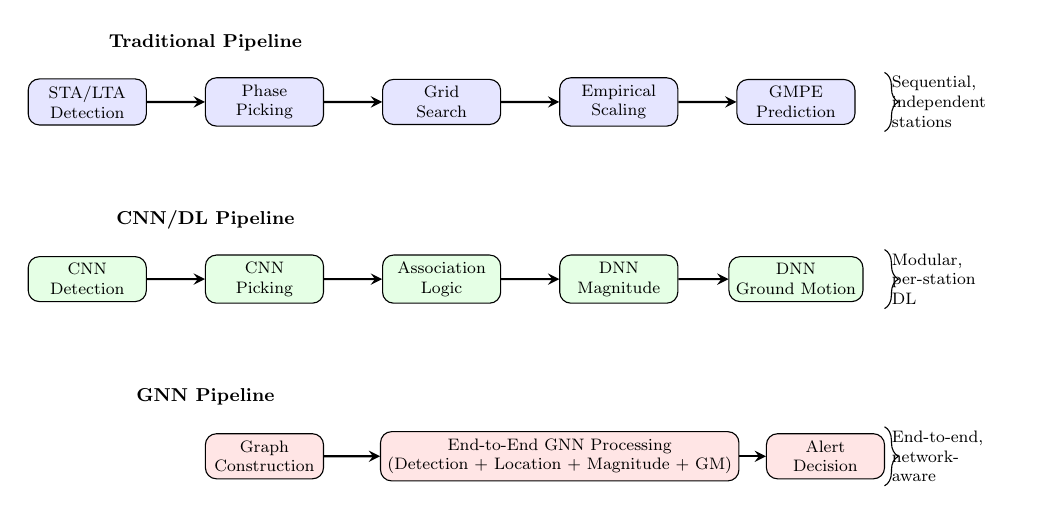
\begin{tikzpicture}[
  tradblock/.style={draw, rounded corners, fill=blue!10, minimum width=2cm, minimum height=0.7cm, align=center, font=\footnotesize},
  mlblock/.style={draw, rounded corners, fill=green!10, minimum width=2cm, minimum height=0.7cm, align=center, font=\footnotesize},
  gnnblock/.style={draw, rounded corners, fill=red!10, minimum width=2cm, minimum height=0.7cm, align=center, font=\footnotesize},
  arrow/.style={->, thick, >=stealth},
  scale=0.75, transform shape
]
  % Traditional Pipeline
  \node[font=\small\bfseries] at (2, 5.5) {Traditional Pipeline};
  \node[tradblock] (t1) at (0, 4.5) {STA/LTA\\Detection};
  \node[tradblock] (t2) at (3, 4.5) {Phase\\Picking};
  \node[tradblock] (t3) at (6, 4.5) {Grid\\Search};
  \node[tradblock] (t4) at (9, 4.5) {Empirical\\Scaling};
  \node[tradblock] (t5) at (12, 4.5) {GMPE\\Prediction};
  \draw[arrow] (t1) -- (t2);
  \draw[arrow] (t2) -- (t3);
  \draw[arrow] (t3) -- (t4);
  \draw[arrow] (t4) -- (t5);
  
  % CNN Pipeline
  \node[font=\small\bfseries] at (2, 2.5) {CNN/DL Pipeline};
  \node[mlblock] (m1) at (0, 1.5) {CNN\\Detection};
  \node[mlblock] (m2) at (3, 1.5) {CNN\\Picking};
  \node[mlblock] (m3) at (6, 1.5) {Association\\Logic};
  \node[mlblock] (m4) at (9, 1.5) {DNN\\Magnitude};
  \node[mlblock] (m5) at (12, 1.5) {DNN\\Ground Motion};
  \draw[arrow] (m1) -- (m2);
  \draw[arrow] (m2) -- (m3);
  \draw[arrow] (m3) -- (m4);
  \draw[arrow] (m4) -- (m5);
  
  % GNN Pipeline
  \node[font=\small\bfseries] at (2, -0.5) {GNN Pipeline};
  \node[gnnblock] (g1) at (3, -1.5) {Graph\\Construction};
  \node[gnnblock, minimum width=5cm] (g2) at (8, -1.5) {End-to-End GNN Processing\\(Detection + Location + Magnitude + GM)};
  \node[gnnblock] (g3) at (12.5, -1.5) {Alert\\Decision};
  \draw[arrow] (g1) -- (g2);
  \draw[arrow] (g2) -- (g3);
  
  % Annotations
  \draw[decorate, decoration={brace, amplitude=5pt}] (13.5, 5) -- (13.5, 4) node[midway, right, font=\footnotesize, text width=2cm] {Sequential,\\independent\\stations};
  \draw[decorate, decoration={brace, amplitude=5pt}] (13.5, 2) -- (13.5, 1) node[midway, right, font=\footnotesize, text width=2cm] {Modular,\\per-station\\DL};
  \draw[decorate, decoration={brace, amplitude=5pt}] (13.5, -1) -- (13.5, -2) node[midway, right, font=\footnotesize, text width=2cm] {End-to-end,\\network-\\aware};
\end{tikzpicture}
\caption{Comparison of processing pipelines: (Top) Traditional seismological pipeline with sequential, independent modules; (Middle) CNN/Deep Learning pipeline replacing individual modules with neural networks but maintaining station-independent processing; (Bottom) GNN-based pipeline enabling end-to-end network-aware processing from graph construction to alert decision.}
\label{fig:pipeline_comparison}
\end{figure}


%% ============================================================
%% SECTION 8: BENCHMARK DATASETS
%% ============================================================
\section{Benchmark Datasets and Evaluation Metrics}
\label{sec:benchmarks}

\subsection{STEAD (Stanford Earthquake Dataset)}

The Stanford Earthquake Dataset (STEAD) \citep{mousavi2019stanford} represents the largest and most widely used benchmark for machine learning in seismology. It contains approximately 1.2 million labeled three-component waveform traces, comprising both earthquake signals and noise recordings from a global distribution of stations and events. Key characteristics include:

\begin{itemize}
  \item \textbf{Scale}: 1,030,232 earthquake waveforms + 100,000 noise traces
  \item \textbf{Coverage}: Events from 135 countries, magnitudes 0--7.9
  \item \textbf{Labels}: P-arrival time, S-arrival time, event parameters (location, magnitude, depth)
  \item \textbf{Format}: Three-component (Z, N, E) 60-second windows at 100~Hz
  \item \textbf{Quality}: Manually reviewed catalog picks with quality metrics
\end{itemize}

For GNN evaluation, STEAD provides individual station traces that must be assembled into network graphs. Researchers typically construct synthetic network scenarios by selecting subsets of traces from events recorded by multiple stations, building graphs with known spatial relationships. The dataset's global coverage enables evaluation of model generalization across diverse tectonic settings, though the artificial graph construction differs from true operational network observations.

\subsection{INSTANCE (Italian Seismic Dataset)}

INSTANCE \citep{michelini2021instance} provides a high-quality regional dataset from the Italian seismic network, offering several advantages for GNN research:

\begin{itemize}
  \item \textbf{Scale}: 1.2 million three-component traces from 50,000+ events
  \item \textbf{Network structure}: Consistent station geometry from the Italian National Seismic Network
  \item \textbf{Metadata}: Complete station coordinates, event catalogs, and quality indicators
  \item \textbf{Tectonic context}: Well-characterized crustal structure with extensive geological information
\end{itemize}

The fixed network geometry of INSTANCE makes it particularly suitable for GNN evaluation, as real graph structures can be constructed from actual station coordinates rather than synthetic configurations. The Italian peninsula's complex tectonics (extension in the Apennines, subduction in the south, compression in the Alps) provide diverse testing scenarios within a single network.

\subsection{LEN-DB and SCEDC}

\textbf{LEN-DB} (Local Earthquakes and Noise Database) \citep{magrini2020lendb} provides a globally compiled dataset of local earthquake recordings with standardized preprocessing, specifically designed for machine learning benchmarking with controlled signal-to-noise conditions.

\textbf{SCEDC} (Southern California Earthquake Data Center) \citep{ross2018scedc} provides access to continuous waveform data from the dense Southern California Seismic Network. Machine learning applied to this dataset has revealed previously undetected events, substantially enriching earthquake catalogs \citep{tan2021machine}. This dataset is particularly valuable for GNN research because:
\begin{itemize}
  \item Dense network geometry (inter-station distances 5--20~km) enables rich graph construction
  \item High seismicity rates provide abundant training data
  \item Well-characterized velocity structure facilitates physics-informed approaches
  \item Historical catalog completeness allows evaluation across magnitude ranges
\end{itemize}

\subsection{Regional Datasets}

Several regional datasets have emerged for specialized EEW research:

\textbf{Japan (Hi-net/K-NET/KiK-net)}: Japan's dense seismic networks provide unmatched station density with $\sim$800 Hi-net (borehole) and $\sim$1,000 K-NET/KiK-net (surface strong motion) stations. This extreme density is ideal for evaluating GNN scalability and the benefits of dense spatial sampling.

\textbf{Chile}: The Chilean Seismological Center maintains records from the subduction zone environment, offering unique challenges including deep events, complex path effects through the subducting slab, and large magnitude ranges.

\textbf{New Zealand (GeoNet)}: New Zealand's GeoNet network provides diverse tectonic environments (subduction, strike-slip, volcanic) within a single monitoring system, enabling multi-domain evaluation.

\subsection{Evaluation Metrics and Protocols}

Standardized evaluation of GNN-based EEW methods requires metrics appropriate to each sub-task:

\textbf{Phase picking}: Residual statistics (mean, standard deviation) between predicted and catalog arrival times; precision, recall, and F1-score for detection with temporal tolerance windows (typically $\pm$0.1--0.5~s).

\textbf{Event detection}: True positive rate, false positive rate, F1-score; detection probability as a function of magnitude and distance (magnitude of completeness).

\textbf{Magnitude estimation}: Root Mean Square Error (RMSE), Mean Absolute Error (MAE), and magnitude-dependent bias analysis; evaluation at different time windows after first detection (1s, 2s, 4s, 8s).

\textbf{Location}: Epicentral distance error (km), depth error (km), combined 3D hypocentral error; comparison against high-precision relative relocations.

\textbf{Ground motion}: Residual analysis against observed values (natural log units), between-event and within-event standard deviations, spatial correlation structure of residuals.

\begin{table}[htbp]
\centering
\caption{Summary of benchmark datasets used for GNN-based seismic analysis evaluation.}
\label{tab:datasets}
\small
\begin{tabular}{p{2cm}p{2cm}ccp{2cm}p{2.5cm}}
\toprule
\textbf{Dataset} & \textbf{Region} & \textbf{Events} & \textbf{Traces} & \textbf{Magnitude Range} & \textbf{Key Features} \\
\midrule
STEAD & Global & 450K+ & 1.2M & 0--7.9 & Large scale, diverse settings \\
INSTANCE & Italy & 50K+ & 1.2M & 0--6.5 & Fixed network geometry \\
LEN-DB & Global & 15K+ & 200K+ & 1--6.5 & Controlled SNR, standardized \\
SCEDC & S. California & 500K+ & 100M+ & $-$0.5--7.3 & Dense network, high rate \\
Hi-net & Japan & 1M+ & 50M+ & 0--9.0 & Extreme density, borehole \\
GeoNet & New Zealand & 100K+ & 10M+ & 0--7.8 & Multi-tectonic domain \\
\bottomrule
\end{tabular}
\end{table}

Critical evaluation considerations for GNN-based methods include: (1) ensuring train/test splits respect temporal ordering (no future data leakage); (2) testing generalization across network configurations not seen during training; (3) evaluating performance degradation under realistic station outage scenarios; and (4) measuring inference latency under operational conditions (including graph construction time).


%% ============================================================
%% SECTION 9: CHALLENGES AND LIMITATIONS
%% ============================================================
\section{Challenges and Limitations}
\label{sec:challenges}

Despite the promising results described in preceding sections, significant challenges must be addressed before GNN-based approaches can achieve widespread operational deployment in EEW systems. This section critically examines these challenges, distinguishing between fundamental limitations inherent to the methodology and practical obstacles that may be overcome through continued research and engineering.

\subsection{Real-time Processing Constraints}

Operational EEW systems impose strict latency requirements: the total processing time from P-wave detection to alert issuance must not exceed 2--4 seconds for the warning to have practical value. This constraint encompasses data acquisition (typically 1~s minimum for sufficient P-wave information), processing (detection, association, parameter estimation), and communication latency.

Current GNN architectures, while faster than many iterative algorithms, still face challenges in meeting these constraints for large networks. A GAT model with 3 attention heads and 3 layers processing 100 stations requires approximately 20--40~ms for inference on GPU hardware (Table~\ref{tab:computational}), which is acceptable. However, practical deployment introduces additional overheads:

\begin{itemize}
  \item Graph construction (computing adjacency matrices, edge features): 5--15~ms
  \item Feature preprocessing (filtering, normalization): 10--20~ms per station
  \item Data assembly from distributed stations: 50--200~ms (network dependent)
  \item Model loading and memory allocation: 100--500~ms (first inference only)
\end{itemize}

Furthermore, EEW systems must process data continuously, not in isolated windows. Streaming GNN architectures that update predictions incrementally as new samples arrive---rather than reprocessing entire windows---remain an active research area. The computational overhead of maintaining and updating graph states in real-time adds complexity beyond batch inference measurements.

\subsection{Scalability to Large Networks}

While GNN computational complexity scales linearly with edge count $O(|\mathcal{E}|)$, the practical scalability to networks with thousands of stations presents challenges:

\textbf{Memory scaling}: Full-batch GNN training on graphs with $>$1000 nodes and dense connectivity requires substantial GPU memory. For networks like Japan's Hi-net ($\sim$800 stations) with $k$-NN connectivity ($k$=20), the graph contains $\sim$16,000 edges per time step, and temporal graphs spanning 10 seconds at 100~Hz multiply this by 1000 time steps.

\textbf{Over-smoothing}: Deep GNN architectures (many layers) suffer from over-smoothing, where node representations converge to indistinguishable values. For seismology, this means that increasing the receptive field to span large networks through additional layers can paradoxically reduce the model's ability to distinguish between stations with different characteristics.

\textbf{Sampling strategies}: Mini-batch training with graph sampling (neighbor sampling, cluster-based sampling) introduces approximation errors that may be unacceptable for safety-critical EEW applications where prediction consistency is paramount.

\subsection{Transfer Learning Across Regions}

A critical practical challenge is the transferability of GNN models trained on one seismic network/region to another with different characteristics:

\textbf{Velocity structure differences}: Seismic wave propagation depends on local crustal velocity structure, which varies dramatically between tectonic settings (oceanic vs. continental, stable vs. active). A model trained on California data implicitly learns California's velocity structure through arrival time patterns, which may not transfer to Japan or Chile.

\textbf{Network geometry differences}: Models trained on dense networks may not perform well on sparse networks, and vice versa. The learned aggregation functions depend on neighborhood statistics that change with station density and distribution.

\textbf{Magnitude distribution differences}: Training data from one region may have different magnitude distributions than the target region. For example, models trained on frequent small earthquakes in California may not generalize to the rare large events that are most critical for EEW in subduction zones.

\citet{yang2023transferlearning} explored transfer learning strategies for GNN-based seismic models, demonstrating that fine-tuning on small amounts of target-region data can partially address these challenges. Transfer learning theory \citep{pan2010survey, weiss2016survey} provides the conceptual foundations for such domain adaptation, yet systematic approaches to domain adaptation for graph-structured seismic data remain underdeveloped.

\subsection{Label Noise and Catalog Quality}

GNN training relies on catalog data (analyst-determined picks, locations, magnitudes) as ground truth labels. However, seismic catalogs contain systematic errors and inconsistencies:

\begin{itemize}
  \item Arrival time picks vary by 0.05--0.2~s between different analysts
  \item Catalog locations have uncertainties of 1--10~km depending on network geometry
  \item Magnitude estimates vary by 0.1--0.3 units between different methods and agencies
  \item Small events near the detection threshold have highly uncertain parameters
\end{itemize}

These label noise effects are particularly problematic for GNN-based methods that aim to achieve sub-second picking precision or sub-kilometer location accuracy---the target precision may exceed the label quality. Self-supervised and contrastive learning approaches that reduce dependence on labeled catalogs represent a promising direction \citep{liu2022graph, chen2020simple}.

\subsection{Interpretability and Explainability}

The deployment of GNN models in safety-critical EEW systems requires that predictions be interpretable and explainable to system operators. Unlike traditional methods where the physical reasoning is explicit (P-wave velocity determines travel time, amplitude scales with magnitude), GNN predictions emerge from complex nonlinear transformations that resist simple interpretation.

Existing GNN explainability methods \citep{ying2019gnnexplainer, lundberg2017unified} can identify important nodes and edges but do not necessarily provide physically meaningful explanations. For seismology, explanations should be expressible in terms of familiar physical quantities (arrival times, amplitudes, frequencies, spatial patterns) rather than abstract neural network features.

The attention weights in GAT-based architectures provide partial interpretability---showing which stations most influence predictions---but do not explain \textit{why} certain stations are weighted more heavily or what features drive the attention pattern \citep{samek2021explaining}. Developing seismologically meaningful interpretation frameworks for GNN-based EEW models remains an open challenge.

\subsection{Robustness to Station Failures}

Operational seismic networks experience frequent data gaps: stations go offline due to equipment failures, telemetry interruptions, power outages, or maintenance. An EEW system must maintain acceptable performance even when a fraction of the network is unavailable.

GNNs offer inherent robustness to missing nodes through their aggregation mechanisms---a station that is offline simply does not contribute messages to its neighbors. However, the degree of graceful degradation under increasing station loss has not been systematically characterized for GNN-based EEW. Critical questions include:

\begin{itemize}
  \item How does performance degrade as a function of the fraction of missing stations?
  \item Are certain stations more critical than others (i.e., do ``key'' stations exist whose removal disproportionately affects network-level predictions)?
  \item Can models be trained to be explicitly robust to random and systematic station outages?
  \item How should confidence/uncertainty estimates reflect reduced network observations?
\end{itemize}

Adversarial robustness---the model's resilience to intentionally manipulated inputs or strategically chosen station removals---is also relevant for critical infrastructure applications, though this remains largely unexplored in the seismological context.


%% ============================================================
%% SECTION 10: FUTURE DIRECTIONS
%% ============================================================
\section{Future Directions}
\label{sec:future}

\subsection{Foundation Models for Seismology}

The concept of foundation models---large-scale models pre-trained on broad data that can be adapted to diverse downstream tasks \citep{bommasani2021opportunities}---is poised to transform seismology. Analogous to how BERT \citep{devlin2019bert} revolutionized natural language processing through self-supervised pre-training, a seismological foundation model would learn general-purpose representations of seismic waveforms and network observations that transfer to phase picking, event detection, magnitude estimation, and EEW with minimal task-specific fine-tuning.

For GNN-based approaches, a foundation model would pre-train graph neural networks on massive amounts of unlabeled continuous seismic data using self-supervised objectives such as:
\begin{itemize}
  \item Masked node prediction: Given partial network observations, predict waveform features at masked stations
  \item Temporal prediction: Given current network state, predict future waveform evolution
  \item Graph contrastive learning: Learn representations where similar seismic events have similar graph embeddings regardless of network geometry
  \item Cross-station consistency: Enforce that representations capture physically meaningful wavefield properties that are consistent across observations from different stations
\end{itemize}

\citet{mousavi2024foundation} outline the opportunities and challenges of machine learning for seismology including emerging foundation model concepts, noting that the diversity of seismic signals (tectonic earthquakes, volcanic tremor, induced seismicity, noise) and the heterogeneity of recording networks present unique challenges compared to language or vision domains.

\subsection{Physics-Informed Graph Neural Networks}

Pure data-driven GNNs learn correlations from training data without guaranteed consistency with physical laws governing seismic wave propagation. Physics-Informed Neural Networks (PINNs) \citep{raissi2019physics} provide a framework for incorporating physical constraints into neural network training, and extending this to graph-structured seismic data represents a high-impact research direction.

Potential physics-informed constraints for GNN-based EEW include:

\textbf{Travel time consistency}: The predicted source location and estimated arrival times at each station must be consistent with seismic wave velocities:
\begin{equation}
\mathcal{L}_{\text{physics}} = \sum_{i \in \mathcal{V}} \left| t_i^{\text{pred}} - \frac{\|\mathbf{x}_{\text{source}} - \mathbf{x}_i\|}{v_P(\text{path}_i)} \right|^2
\end{equation}

\textbf{Amplitude decay}: Predicted amplitudes must respect geometric spreading and attenuation:
\begin{equation}
A_i \propto \frac{1}{R_i} \cdot \exp(-\pi f R_i / Q v)
\end{equation}
where $R_i$ is hypocentral distance, $f$ is frequency, and $Q$ is the quality factor.

\textbf{Waveform coherence}: Signals at nearby stations should exhibit predictable coherence patterns determined by the wavefield's spatial correlation length.

\textbf{Conservation laws}: Energy partitioning between P, S, and surface waves must respect physical constraints, and total radiated energy must be consistent with estimated magnitude.

Approaches by \citet{rasht2022physics}, \citet{smith2022hyposvi}, and \citet{moseley2020solving} demonstrate the feasibility of physics-informed deep learning for earthquake location and wave equation solving, suggesting that analogous constraints can improve GNN-based models while providing physical plausibility guarantees essential for operational trust.

\subsection{Federated Learning for Distributed Seismic Networks}

Seismic monitoring data is distributed across national agencies, research institutions, and private operators who may be unable or unwilling to share raw waveform data due to data sovereignty regulations, intellectual property concerns, or bandwidth limitations. Federated learning \citep{mcmahan2017communication, li2020federated} enables collaborative model training without data centralization, maintaining data at its source while sharing only model updates.

A federated GNN-based EEW system would:
\begin{enumerate}
  \item Train local GNN models on each agency's network data
  \item Share model parameters (or gradients) with a central coordinator
  \item Aggregate updates to produce a global model that benefits from all participants' data
  \item Return the improved global model to each participant for local deployment
\end{enumerate}

Challenges specific to federated learning in seismology include:
\begin{itemize}
  \item Non-IID data distributions (different tectonic settings produce different event characteristics)
  \item Heterogeneous network geometries requiring architecture adaptation
  \item Asynchronous data availability (some networks have decades of data, others are recently deployed)
  \item Communication efficiency for large graph models
\end{itemize}

\subsection{Multi-modal Data Fusion}

EEW systems have traditionally relied exclusively on seismometer data, but complementary geodetic and remote sensing observations could significantly enhance performance, particularly for large events:

\textbf{GNSS (Global Navigation Satellite System)}: Real-time GNSS provides direct measurement of ground displacement, unclipped by sensor limitations. For M$>$7 events, GNSS-detected static offsets and dynamic displacements provide magnitude constraints that seismometers cannot achieve alone \citep{gualandi2017geodetic}.

\textbf{InSAR (Interferometric Synthetic Aperture Radar)}: While not real-time, InSAR-derived deformation maps can inform GNN models through training data augmentation and provide ground truth for large earthquake characterization.

\textbf{Distributed Acoustic Sensing (DAS)}: Fiber-optic DAS transforms existing telecommunication cables into dense sensor arrays with meter-scale spacing \citep{zhu2023seismic}. Integrating DAS measurements into GNN-based EEW requires handling extremely dense ``stations'' (nodes) with lower sensitivity but unprecedented spatial resolution. Recent work on graph-based rapid waveform modeling further demonstrates the potential of GNNs for processing dense array data \citep{li2023das}.

\textbf{Multi-modal GNN architectures}: Fusing heterogeneous sensor types into a unified graph requires heterogeneous graph neural networks where different node types (seismometer, GNSS, DAS channel) have different feature dimensions and different edge types encode different physical relationships \citep{baltrusaitis2019multimodal}.

\subsection{Edge Computing and On-device Inference}

Deploying GNN inference at network edge devices (at or near seismic stations) rather than centralized data centers could dramatically reduce communication latency---the single largest contributor to EEW delay in many deployments. Edge deployment requires:

\begin{itemize}
  \item Model compression: Pruning, quantization, and knowledge distillation to fit GNN models on embedded hardware \citep{shi2016edge, chen2019deep}
  \item Partial graph inference: Running subgraph-level GNN inference locally, communicating only compact node embeddings rather than raw waveforms
  \item Hierarchical architecture: Local nodes perform preliminary detection and feature extraction; regional hubs aggregate multi-station graphs for refined estimation
  \item Hardware co-design: Custom accelerators optimized for sparse graph operations on low-power platforms
\end{itemize}

\subsection{Self-supervised and Contrastive Learning}

Reducing dependence on labeled catalogs through self-supervised learning represents a key direction for expanding GNN-based EEW to data-rich but label-poor scenarios. Contrastive learning approaches \citep{chen2020simple} can learn discriminative representations by contrasting different views of seismic data:

\begin{itemize}
  \item \textbf{Spatial augmentation}: Different subgraph views of the same event provide positive pairs
  \item \textbf{Temporal augmentation}: Different time windows of the same event provide positive pairs
  \item \textbf{Cross-network views}: The same event recorded by overlapping networks provides natural augmentation
\end{itemize}

\citet{liu2022graph} review self-supervised graph learning methods that can be adapted to seismic applications, while \citet{zhu2023seismic} demonstrate semi-supervised approaches for seismic phase picking that achieve near-supervised performance with only 10\% labeled data.

\begin{figure}[htbp]
\centering
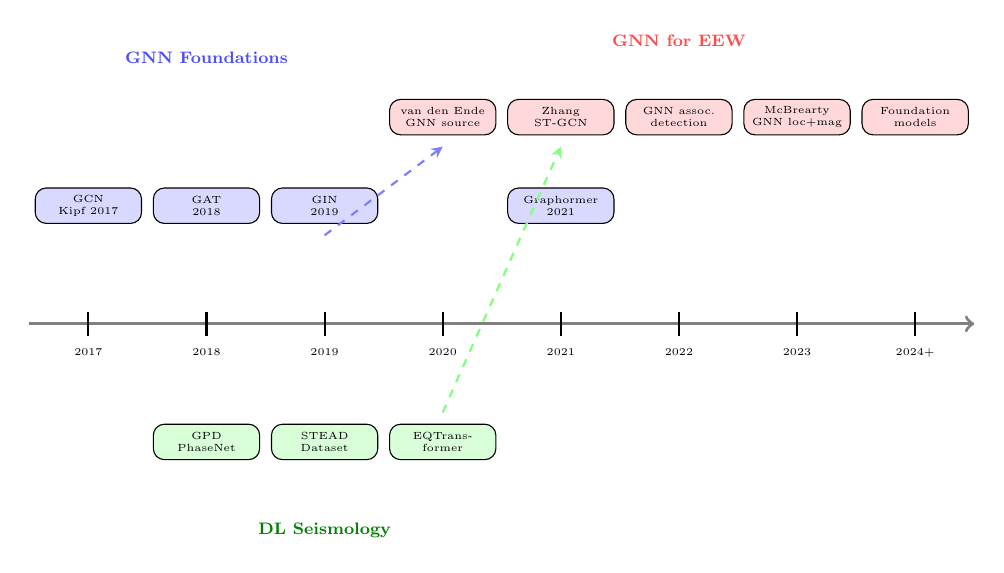
\begin{tikzpicture}[
  milestone/.style={draw, rounded corners, fill=white, minimum width=1.8cm, minimum height=0.6cm, align=center, font=\tiny},
  era/.style={draw, rounded corners, fill=blue!8, minimum width=3cm, minimum height=1.2cm, align=center, font=\footnotesize},
  arrow/.style={->, thick, >=stealth},
  scale=0.75, transform shape
]
  % Timeline
  \draw[->, very thick, gray] (0, 0) -- (16, 0);
  
  % Year markers
  \foreach \x/\y in {1/2017, 3/2018, 5/2019, 7/2020, 9/2021, 11/2022, 13/2023, 15/2024+} {
    \draw[thick] (\x, -0.2) -- (\x, 0.2);
    \node[font=\tiny, below] at (\x, -0.3) {\y};
  }
  
  % Milestones - GNN development
  \node[milestone, fill=blue!15] at (1, 2) {GCN\\Kipf 2017};
  \node[milestone, fill=blue!15] at (3, 2) {GAT\\2018};
  \node[milestone, fill=blue!15] at (5, 2) {GIN\\2019};
  \node[milestone, fill=blue!15] at (9, 2) {Graphormer\\2021};
  
  % Milestones - Seismology DL
  \node[milestone, fill=green!15] at (3, -2) {GPD\\PhaseNet};
  \node[milestone, fill=green!15] at (5, -2) {STEAD\\Dataset};
  \node[milestone, fill=green!15] at (7, -2) {EQTrans-\\former};
  
  % Milestones - GNN+Seismology
  \node[milestone, fill=red!15] at (7, 3.5) {van den Ende\\GNN source};
  \node[milestone, fill=red!15] at (9, 3.5) {Zhang\\ST-GCN};
  \node[milestone, fill=red!15] at (11, 3.5) {GNN assoc.\\detection};
  \node[milestone, fill=red!15] at (13, 3.5) {McBrearty\\GNN loc+mag};
  \node[milestone, fill=red!15] at (15, 3.5) {Foundation\\models};
  
  % Era labels
  \node[font=\footnotesize\bfseries, blue!70] at (3, 4.5) {GNN Foundations};
  \node[font=\footnotesize\bfseries, green!50!black] at (5, -3.5) {DL Seismology};
  \node[font=\footnotesize\bfseries, red!70] at (11, 4.8) {GNN for EEW};
  
  % Arrows connecting eras
  \draw[arrow, blue!50, dashed] (5, 1.5) -- (7, 3);
  \draw[arrow, green!50, dashed] (7, -1.5) -- (9, 3);
\end{tikzpicture}
\caption{Timeline of key developments at the intersection of Graph Neural Networks and seismology (2017--2024+). The convergence of GNN architectural advances (top), deep learning in seismology (bottom), and their intersection (middle) has accelerated since 2020, with operational GNN-EEW systems anticipated by 2025--2026.}
\label{fig:timeline}
\end{figure}


%% ============================================================
%% SECTION 11: ETHICAL AND OPERATIONAL CONSIDERATIONS
%% ============================================================
\section{Ethical and Operational Considerations}
\label{sec:ethical}

\subsection{False Alert Management and Public Trust}

The societal value of an EEW system depends fundamentally on public trust, which is eroded by false alerts and missed events. The deployment of GNN-based models introduces new dimensions to false alert management:

\textbf{Model uncertainty quantification}: Unlike threshold-based systems where the trigger logic is transparent, GNN predictions require rigorous uncertainty quantification to support alert decisions. Bayesian GNN variants, ensemble methods, or Monte Carlo dropout can provide uncertainty estimates, but these must be calibrated against operational requirements (e.g., no more than 1 false alert per year above a given severity threshold).

\textbf{Graceful failure modes}: When a GNN model encounters inputs far from its training distribution (e.g., a previously unseen event type, an unusual noise pattern), the system must fail gracefully---issuing conservative predictions with large uncertainty rather than confidently wrong estimates. Out-of-distribution detection mechanisms are essential but challenging for graph-structured data.

\textbf{Human oversight}: Even with high model accuracy, operational EEW systems require human oversight and override capabilities. The ``human-in-the-loop'' paradigm must be adapted for the extreme time pressure of EEW, where decisions must be made in 1--3 seconds. GNN interpretability tools that can provide instant visual explanations of alert decisions would support rapid human verification.

\textbf{Public communication}: Explaining GNN-based alert decisions to the public (``why did I receive/not receive an alert?'') requires translating complex model outputs into accessible narratives. This is more challenging for end-to-end GNN systems than for modular traditional pipelines where each step has a clear physical interpretation.

\subsection{Equity in EEW Coverage}

The distribution of seismic monitoring infrastructure globally reflects historical economic disparities: developed nations maintain dense networks with thousands of stations, while many developing countries with high seismic risk have sparse or absent monitoring. GNN-based methods have implications for equity:

\textbf{Potential benefits}: GNNs that perform well on sparse networks could enable EEW in regions with limited infrastructure. Transfer learning from data-rich regions to data-poor regions could accelerate system deployment. Low-cost sensor networks combined with sophisticated GNN processing could democratize EEW access.

\textbf{Potential risks}: If GNN models are predominantly trained on data from well-instrumented regions, they may exhibit systematic biases when deployed elsewhere. The computational resources required for GNN training and deployment may be inaccessible to institutions in resource-limited settings.

\textbf{Recommendations}: International collaboration should prioritize open-source GNN models pre-trained on global data, with adaptation protocols for regional deployment. Lightweight model architectures suitable for resource-constrained environments should be developed alongside high-performance variants.

\subsection{Model Governance and Continuous Validation}

The lifecycle management of GNN-based EEW models requires governance frameworks addressing:

\textbf{Model versioning}: As models are retrained with new data, performance characteristics may change. Rigorous version control and regression testing must ensure that updates improve performance without introducing new failure modes.

\textbf{Continuous monitoring}: Deployed models must be monitored for performance degradation over time (concept drift), which could arise from network changes (new stations, decommissioned stations), evolving seismicity patterns, or gradual sensor degradation.

\textbf{Validation against ground truth}: Post-event analysis must systematically compare GNN predictions against final, reviewed source parameters. Discrepancies should trigger model investigation and potential retraining.

\textbf{Regulatory compliance}: As EEW systems are increasingly linked to automated protective actions (shutting down trains, opening fire station doors, initiating building responses), the regulatory requirements for model validation and certification will intensify. Clear standards for GNN model validation in safety-critical applications are needed.

\subsection{Integration with Emergency Response Systems}

GNN-based EEW outputs must interface with downstream emergency response infrastructure:

\begin{itemize}
  \item Building response systems (elevator control, gas shutoff, structural dampers)
  \item Transportation management (train deceleration, traffic signal control)
  \item Industrial process protection (nuclear facility shutdown, chemical plant safety systems)
  \item Public alert dissemination (smartphone notifications, broadcast interruptions, sirens)
  \item Hospital and healthcare facility preparation
\end{itemize}

Each downstream system has specific requirements for alert format, confidence level, lead time, and false alert tolerance. GNN-based EEW systems must provide standardized output interfaces with calibrated probability estimates that downstream decision systems can interpret within their own risk frameworks. The development of such standardized interfaces between AI-driven seismic analysis and automated response systems represents an important area for future standardization efforts.

%% ============================================================
%% SECTION 12: CONCLUSIONS
%% ============================================================
\section{Conclusions}
\label{sec:conclusions}

This review has presented a comprehensive examination of Graph Neural Networks as applied to Earthquake Early Warning systems, spanning theoretical foundations, current applications, comparative analyses, challenges, and future directions. The key findings and conclusions are:

\textbf{GNNs provide a natural computational framework for seismic network data.} The representation of monitoring networks as graphs---with stations as nodes and spatial/physical relationships as edges---enables explicit modeling of inter-station correlations that are fundamental to seismological analysis but inaccessible to station-independent methods. This representational advantage translates to measurable performance improvements across EEW tasks including phase picking, source characterization, magnitude estimation, and ground motion prediction.

\textbf{Current GNN-based methods demonstrate significant improvements over traditional approaches.} Comparative analyses show that GNN architectures achieve approximately 15--30\% reduction in magnitude estimation error and 20--40\% improvement in location accuracy as reported across recent studies \citep{mcbrearty2023earthquake, vandenende2020automated, bloemheuvel2022graph, jozinovic2022ground}, with enhanced detection sensitivity for small events, relative to conventional methods. These improvements are most pronounced for sparse network scenarios and complex multi-event sequences, precisely the conditions where traditional methods struggle most.

\textbf{Temporal-spatial GNN formulations are essential for EEW.} The inherently dynamic nature of seismic wavefield propagation requires architectures that jointly model spatial (inter-station) and temporal (intra-waveform) patterns. Dynamic graph approaches that progressively incorporate stations as P-waves arrive align naturally with the sequential decision-making of operational EEW, achieving the most promising performance among GNN variants.

\textbf{Significant challenges remain before operational deployment.} Real-time processing constraints, transfer learning across tectonic regions, interpretability requirements, and robustness to station failures represent active research frontiers. The gap between research demonstrations (typically evaluated on curated benchmarks) and operational deployment (requiring 24/7 reliability, calibrated uncertainty, and graceful failure modes) should not be underestimated.

\textbf{Future directions point toward transformative capabilities.} The convergence of foundation models, physics-informed learning, federated training, multi-modal fusion, and edge computing promises GNN-based EEW systems that are more accurate, faster, more robust, and more broadly deployable than any current system. Physics-informed GNNs that embed seismic wave propagation constraints offer particular promise by combining data-driven flexibility with physical plausibility guarantees.

\textbf{Recommendations for researchers}:
\begin{enumerate}
  \item Develop standardized benchmarks specifically designed for network-level (graph-based) seismic processing, complementing existing station-level datasets.
  \item Invest in interpretability methods that translate GNN decisions into seismologically meaningful explanations.
  \item Pursue physics-informed architectures that embed wave equation constraints into graph learning.
  \item Address the transfer learning challenge through domain adaptation methods and globally pre-trained foundation models.
  \item Establish latency benchmarks under realistic operational conditions, not just batch inference measurements.
\end{enumerate}

\textbf{Recommendations for practitioners}:
\begin{enumerate}
  \item Begin integration of GNN components into existing EEW pipelines incrementally, starting with phase association and source characterization modules where GNN advantages are most clearly demonstrated.
  \item Maintain traditional methods as fallback systems during GNN deployment, establishing confidence through parallel operation before full transition.
  \item Develop robust model monitoring and validation frameworks before operational deployment of any data-driven EEW component.
  \item Engage with the machine learning research community through shared datasets, open-source implementations, and collaborative benchmarking efforts.
\end{enumerate}

The intersection of graph neural networks and earthquake early warning represents one of the most promising frontiers in computational seismology. While fundamental challenges remain, the pace of progress suggests that GNN-based methods will become integral components of next-generation EEW systems within the coming decade, contributing to the reduction of earthquake losses through faster, more accurate, and more robust early warning capabilities.

\section*{Acknowledgments}

The authors received no specific funding for this review article. We thank the developers of STEAD, INSTANCE, and SeisBench for making benchmark datasets publicly available, and the global seismological community for maintaining open data archives that enable machine learning research in earthquake science.

\section*{Declaration of Competing Interest}

The authors declare that they have no known competing financial interests or personal relationships that could have appeared to influence the work reported in this paper.

\section*{Data Availability}

No new data were generated in this review article. All referenced datasets (STEAD, INSTANCE, LEN-DB, SCEDC) are publicly available through their respective data repositories.

\bibliographystyle{elsarticle-harv}
\bibliography{references}

\end{document}
